\newtheorem{definition}{\textbf{Definice}}

\chapter{Úvod}
\label{ch:uvod}

V~dnešní době je obor umělé inteligence (AI) stále více všudypřítomný a~jeho působení ovlivňuje mnoho aspektů našeho života.

Pokrok umělé inteligence je dobře měřitelný jejím aplikováním v~oblasti her.
Protože právě hry nabízí jasně definovaná pravidla a~cíle, čímž se stávají ideálním testovacím prostorem pro algoritmy umělé inteligence.
Výkon AI je ve hrách snadno měřitelný a~pokrok dokáže vidět i~laik bez žádných složitých grafů, tabulek a~výpočtů.
Umělá inteligence již dokázala porazit nejlepší hráče v~\textit{šachu}~\cite{DeepBlue}, \textit{Dota 2}~\cite{Dota2}, \textit{Go}~\cite{AlphaGo} a~spoustě dalších her.


Hra studovaná v~této práci se jmenuje \emph{Scotland Yard}.
Jedná se o~hru pro tři až šest hráčů.
V~této hře obvykle hraje jeden hráč jako Pan~X, který se pokouší uniknout policistům ovládaným ostatními hráči.
Policisté však nevědí, kde na herním poli se Pan~X nachází.
Musí tedy odhadovat jeho pozici a~spolupracovat mezi sebou, aby ho mohli polapit.
Pozice Pana~X je policistům odhalena pouze v~určitých kolech.
Scotland Yard je ideální hrou ke studování neurčitosti ve hrách hraných systémy umělé inteligence, protože se jedná o~hru s~nedokonalou informací a~k~vítězství policistů je zapotřebí spolupráce, strategie a~odhadování.

Tato práce zkoumá algoritmy posilovaného učení, jejich použití na hry s~neurčitostí a~jejich porovnání s~klasickými metodami hraní her.
Algoritmus optimalizace proximální strategie (Proximal Policy Optimization --- PPO) je hlavním zkoumaným algoritmem této práce.
PPO je často používán k~řešení problémů se spojitými veličinami a~ve 3D prostoru.
Pro srovnání s~jinými algoritmy slouží algoritmus Deep-Q-Learning (DQN).
Výslední agenti\footnote[1]{V kontextu se hrou Scotland Yard je důležité nezaměňovat agenta za policistu.
Význam pojmu \emph{agent} je popsáno v~kapitole \nameref{subsec:agent}} byli také testováni proti hráči, který náhodně vybírá své akce.

Algoritmus PPO byl vybrán z~důvodu jeho úspěšnosti při použití ve složitých hrách s~neurčitostí.
Toto tvrzení podporuje experiment OpenAI~\cite{PPO_Hide_Seek_page}, podrobně popsán zde~\cite{PPO_Hide_Seek_paper}.
V~tomto experimentu byla optimalizace proximální strategie použita pro učení strategie ve hře typu \textit{schovávaná} s~několika agenty a~neúplnou informací.
Jelikož tento typ hry přesně odpovídá i~hře Scotland Yard, zdá se být vhodný i~pro řešení této hry.
Také další studie~\cite{Manille} a~\cite{Dota2} tento výrok dále podporují a~dokazují vhodnost algoritmu PPO pro tuto práci.

Zaměření této práce jsem si vybral, protože je mi obor umělé inteligence blízký a~vždy jsem se chtěl začít tomuto odvětví více věnovat i~po praktické stránce.
Algoritmus PPO je pro mě zajímavý a~zkušenost s~ním by se dala využít v~mém dalším pracovním životě.\newpage

Pro zpracování práce byly využity tyto hlavní knihovny:
\begin{myitemize}
  \item \texttt{Ray.Rlib} --- framework pro posilované učení.
  Obsahuje již zhotovenou implementaci algoritmu PPO a~DQN, které byly použity v~této práci.

  \item \texttt{PyTorch} --- podpůrná knihovna \texttt{Ray.Rlib}
  \item \texttt{Gymnasium} --- knihovna použita k~vytvoření prostředí hry Scotland Yard
  \item \texttt{Pygame} --- knihovna pro vytváření uživatelského rozhraní
\end{myitemize}

Práce byla zhotovena pro operační systémy Windows a~Python verze 3.10

\chapter{Teoretický základ}
\label{ch:teoreticky_zaklad}
Tato kapitola není encyklopedickým přehledem celého tématu bakalářské práce.
Ale jedná se o~shrnutí nejdůležitějších relevantních informací a~pojmů, důležitých pro tuto práci.

\section{Desková hra Scotland Yard}
\label{sec:deskova-hra-scotland-yard}

Scotland Yard je populární hra pro tři a~více hráčů, která kombinuje prvky schovávané a~hry na honěnou.
Jeden hráč hraje za Pana~X, který se snaží uniknout policistům, kteří jsou ovládáni zbylými hráči.
Hra je u~konce, pakliže je Pan~X úspěšně chycen policisty (vyhrávají policisté), nebo když je dosaženo maximálního počtu kol, bez toho, aniž by byl Pan X chycen (vyhrává Pan~X).
Originální hra se odehrává na mapě Londýna.

\begin{figure}[H]
	\centering
	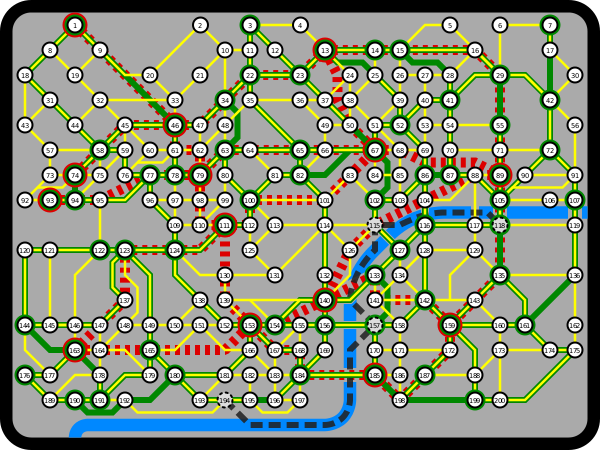
\includegraphics[width=0.87\textwidth]{obrazky-figures/scotland_original}
	\caption{Ukázka herní mapy hry Scotland Yard.
  Zdroj~\cite{scotland_original_image}:}\label{fig:figure}
\end{figure}
\newpage

Na této herní mapě se nachází 200 polí, která jsou vzájemně propojená cestami.
Každá z~těchto cest povoluje pouze určitý způsob dopravy (např.
pouze taxíkem, pouze autobusem atd.).
Jednotliví hráči využívají prvky veřejné dopravy k~pohybu po herní ploše, kterými jsou:

\begin{myitemize}
  \item \emph{Taxi};
  \item \emph{Autobus};
  \item \emph{Metro};
  \item \emph{Trajekt}.
\end{myitemize}

Každému hráči je na začátku hry přidělen pouze určitý počet jízdenek na tyto typy dopravních prostředků.
K~využití dopravy je použita právě tato jízdenka.
Pokud již hráč nemá některou z~jízdenek, nemůže nadále tento způsob přepravy využívat.
Hra se dělí na kola, ve kterých se hráči postupně střídají.
Jakmile Pan X provede svůj tah, je odhaleno pouze to, jaký typ dopravy využil, ale neodhaluje, na které místo se přemístil.

Hlavní myšlenkou hry je, že po většinu kol je pozice Pana~X policistům utajena.
Odhaluje se jim pouze určená kola.
To znamená, že policisté pro polapení Pana~X musí odhadovat jeho pozici a~spolupracovat mezi sebou.
Tímto se ze hry Scotland Yard stává hra s~nedokonalou informací, jelikož policisté nevidí přesnou pozici Pana~X\@.
Tento fakt ji činí vhodnou pro studování metod hraní her s~neurčitostí.

Pan X má také možnost použít speciální akci, kterou je \emph{dvojitý tah}, a~také vlastní speciální jízdenku, která mu umožňuje použít jakýkoliv druh dopravy.
Pokud Pan X použije tuto speciální jízdenku, není policistům odhalen, jaký typ dopravy využil.

\section{Další hry s~nedokonalou informací a~systémy využívající algoritmus PPO}\label{sec:dalsi-hry-s-nedokonalou-informaci}
V~oblasti umělé inteligence hraje důležitou roli modelování a~řešení her.
Hry představují formalizaci konfliktních interakcí mezi aktéry.
Klasická teorie her se zaměřuje na hry s~úplnou informací, kde mají všechny strany v~daném okamžiku přístup ke všem relevantním informacím z~herního prostředí.
Znají strategie a~cíle ostatních hráčů.
V~praxi se však častěji setkáváme se situacemi, kde jednotlivým stranám chybí některé informace, ať už se jedná o~informace z~prostředí či cíle soupeře.

Následující hry byly vybrány pro svou složitost a~neúplnou informaci, kterou obsahují.
V~obou případech byly prokázány dobré výsledky s~použitím algoritmu PPO.
Na základě těchto výsledků i~já zvolil algoritmus PPO pro řešení hry Scotland Yard.

\subsection{Dota 2}\label{subsec:dota}
Dota 2 je velmi komplexní strategická hra odehrávající se v~reálném čase.
Hraje se ve dvou týmech po pěti hráčích, kteří ovládají postavy s~různými unikátními schopnostmi.
Schopnosti jsou hlavní součástí hry.
Díky schopnostem mohou hrdinové zranit nepřítele, udělat silnější sebe či své spojence a~mohou mít i~spoustu dalších efektů.
Co jim navíc přidává na komplexnosti, je to, že každá schopnost nemůže být po použití znovu použita po určitou dobu.

Ve hře se vyskytuje válečná mlha, která způsobuje, že hráči vidí pouze část mapy ve svém okolí a~okolí spřátelených jednotek.
To znamená, že nemají úplnou informaci o~pozici nepřátelských jednotek.

\bigskip

Dota 2 je pro umělou inteligenci náročnou výzvou z~těchto důvodů:
\begin{myitemize}
  \item Složitost hry

  Její stav se mění velmi rychle, a~je tedy těžké předpovídat vývoj hry.
  Agenti tedy musí být schopni rychle reagovat na změny a~přizpůsobit jim svoji strategii.

  Pozorovací prostor je obrovský, obsahuje až 16 000 vstupů.
  Akční prostor je složitý, jelikož lidé hrají Dotu 2 většinou pomocí myši a~klávesnice.
  U~OpenAI Five je akční prostor rozdělen na hlavní akce a~jejich parametry.
  Hlavní akce jsou například pohyb, útok, použití schopnosti/ předmětu, zakoupení předmětu a~další situační akce.
  Dostupnost těchto akcí je závislá na stavu hry a~je řízena maskou akcí.
  Tyto akce mají 3 parametry - zpoždění, vybranou jednotku a~offset cíle akce.
  Pokud se tyto akce a~jejich parametry zkombinují, výsledkem je 1 837 080 možných akcí.

  \item Nedokonalá informace

  Právě kvůli válečné mlze nemají hráči úplnou informaci o~pozici nepřátelských jednotek, a~musí tedy pouze odhadovat, kde na mapě se nachází.
  Nevědí ani, jestli jsou nepřátelé schopni použít své schopnosti a~předměty.
  Ve hře dota 2 vykonávají hráči několik rozhodnutí někdy i~několikrát za sekundu.
\end{myitemize}

Dota 2 sama o~sobě obsahuje implementaci chování inteligentních agentů, kteří jsou schopni hrát hru na velmi vysoké úrovni.
Jejich výkon však není dostatečný a~nebyli schopni ani zdaleka porazit zkušené.
Použité metody pro vytvoření těchto agentů bohužel nejsou zveřejněny.

Inovaci umělé inteligence v~této hře opět přinesla společnost OpenAI a~jejich projekt \emph{OpenAI Five}~\cite{Dota2}.
Tento projekt se zaměřil na vytvoření modelu, který by byl schopen porazit nejlepší hráče světa ve hře Dota 2.
OpenAi zvolila pro učení výsledného modelu algoritmus \textbf{PPO}.
Agent OpenAI Five byl kombinovaně s~předchozí verzí trénován asi \emph{55~000} herních let hraním sama proti sobě metodou self-play.

I~přes velikost hry je výsledný reakční čas agenta okolo 33~ms, oproti tomu reakční čas profesionálních hráčů her je okolo 120~ms~\cite{reaction_time}.
OpenAi Five porazil tehdejší nejlepší tým světa během exhibice na nejprestižnějším turnaji Dota2 \textit{The International}.
V~celém exhibičním turnaji proti nejlepším týmům světa z~celkových 24 her vyhrál 19 her a~pouhých 5 prohrál.

\subsection{Experiment OpenAI}\label{subsec:experiment-openai}
Důležitým zdrojem pro tuto práci byla studie~\cite{PPO_Hide_Seek_paper} od společnosti OpenAI.
Z~ní vyplývá, že algoritmus \textbf{PPO} je vhodný pro řešení problémů s~nedokonalou informací.
V~dané studii byl algoritmus implementován na komplexní hru typu schovávaná.
Ve hře proti sobě hrají dva typy hráčů.
Modří hráči se snaží schovat a~utéct před červenými.
Po herní ploše byly rozestavěny objekty, se kterými hráči mohou interagovat.
Mohou je přesouvat a~následně \uv{zamrazit} na místě, takže s~objektem nelze pohybovat.
Modří hráči se na začátku hry objevují ve své pevnosti, která má několik děr.
Červeným hráčům je na začátku hry znemožněn pohyb, což dává modrým hráčům čas připravit se na jejich útok.

Po více než 8 miliónech epizodách učení se modří hráči naučili efektivně blokovat vstup do své pevnosti, takže je červení hráči nebyli schopni dostihnout.
Červení hráči se poté adaptovali a~naučili se využívat rampy a~přelézt opevnění modrých hráčů.
Finální strategii se modří naučili po 43 miliónech epizod.
Modří hráči na začátku kola ukradli červeným všechny rampy a~zabarikádovali se i~s~nimi v~pevnosti.
Červení hráči tak neměli žádnou šanci na výhru.

Dokonce se objevily i~fascinující strategie, které zneužívaly chyby v~prostředí.
Například v~kódu obsluhující kolize byla chyba, která způsobovala, že při najetí rampy na zeď arény pod určitým úhlem byla rampa rapidní rychlostí vymrštěna do vzduchu.
Toho červení hráči zneužili a~za pomoci této chyby se vymršťovali do vzduchu, aby překonali zdi pevnosti modrých.

\section{Klíčové koncepty posilovaného učení}\label{sec:klicove-koncepty-posilovaneho-uceni}
Posilované učení (Reinforcement Learning, RL) je oblast strojového učení, která se zaměřuje na učení agentů v~dynamickém prostředí.
Agent se učí strategii chování, která maximalizuje kumulativní odměnu.

\subsection{Agent}\label{subsec:agent}
Agent je komplexní entita, která interaguje s~prostředím.
Prostředí poskytuje agentovi informace o~stavu a~agent na základě těchto pozorování a~své strategie vykonává akce.
Ty mohou ovlivnit stav prostředí a~agent obdrží odměnu na základě odměnové funkce.

Na základě těchto odměn se agent učí, které akce jsou vhodné, které naopak ne, a~upravuje model podle své strategie.
Agent většinou volí takové akce, aby maximalizoval kumulativní odměnu.

Pro textový obsah této práce je velmi důležité definovat pojem \emph{agent}.
Slovo je podobné slovu \emph{policista}, a~v~kontextu hry Scotland Yard je tedy možné tyto významy zaměnit.\\
\emph{Slovo agent v~této práci výhradně označuje entitu, která je zde popsána, a~nikde nevystupuje jako synonymum ke slovu policista.}

\subsection{Pozorovací a~akční prostor}
\label{subsec:prostory}

\textbf{Pozorovací prostor} je jednou z~nejdůležitějších součástí posilovaného učení.
Bez jeho vhodného zvolení je dosažení strategie s~dobrými výsledky velmi obtížné.
Pozorovací prostor je množina všech možných pozorování, která může agent získat z~prostředí.
Je to tedy forma, kterou prostředí předává informace agentovi.
Velmi často se aktuální stav pozorovacího prostoru využívá jako stav.
Při vytváření prostředí je nutné definovat typ, tvar prostoru a~jakých hodnot může nabývat.

Pro jeho podobu je vhodné zvolit standard z~knihovny \texttt{Gymnasium}~\cite{Gymnasium}.
Gymnasium je pokračování knihovny \texttt{Gym} od společnosti OpenAI\@.
Tyto knihovny nastavily standard vytváření prostředí pro posilované učení.
Dodržování těchto standardů umožňuje použití libovolného algoritmu na jedno prostředí.

\bigskip

\textbf{Akční prostor} je, jak název vypovídá, množina všech možných akcí, ze kterých může strategie volit.
Často se jedná o~konečnou množinu celočíselných hodnot, které reprezentují různé akce.
Samozřejmě může být akční prostor i~spojitého typu (blíže popsáno v~další sekci).

V~herním prostředí mohou nastat situace kdy se nějaká akce stane nevalidní, jelikož by její provedení vyústilo v~nevalidní stav herního prostředí.
V~takovém případě je vhodné zvolení této akce zamezit, nejlépe pomocí akční masky.
Ta definuje, které akce jsou v~momentálním stavu prostředí proveditelné.
Lze také tyto akce povolit, ale následně agentovi udělit sníženou odměnu za provedení nevalidní akce.

\subsection{Diskrétní a~spojitý prostor}\label{subsec:diskretni-a-spojity-prostor}

Je-li prostor \textbf{diskrétní}, je konečný nebo spočetně nekonečný.

Příkladem takového prostoru je například pozorovací prostor, jehož vstupem je fotka.
Ta se dělí na přesně daný počet pixelů, kde každý má dané hodnoty RGB.\@
Diskrétní akční prostory jsou spočetné a~často se jedná o~konečnou množinu možných akcí.
Například akce pohybu \textit{vlevo}, \textit{vpravo}, \textit{nahoru} a~\textit{dolů}.

Zato \textbf{spojitý prostor} je nekonečný a~nespočetný.

Spojitý pozorovací prostor je například pozice robota ve 3D prostoru, nebo jeho rychlost.
Spojitý akční prostor může například ovládat sílu stlačení pedálu nebo úhel natočení kola.

\subsection{Prostředí}\label{subsec:prostredi2}

Je vše, s~čím agent interaguje.
Prostředí je buď fyzické (entity z~reálného světa, ovládání chytré domácnosti, robotické ruky, ovládání reaktoru apod.), nebo virtuální (simulace nebo hra).
Prostředí reaguje na zvolené akce agenta, poskytuje mu zpětnou vazbu ve formě odměny.
Odměna může být i~záporná, pokud agent zvolil velmi nevhodnou akci.
Pokud v~prostředí existuje více agentů, může mít každý agent jiné pozorování.
Díky tomu můžeme například schovat agentovi \textit{A} určité informace, které agent \textit{B} vidí.

\subsection{Strategie (Policy)}\label{subsec:strategie}

Pomocí posilovaného učení vzniká strategie.
Strategie je matematická funkce, která definuje agentovo chování na základě jeho pozorování (stavu).
Snaží se definovat takové chování, které vede k~maximální kumulativní odměně.
Strategie může být deterministická, nebo stochastická.

  \subsubsection*{Deterministická strategie}
  
  Deterministická strategie přesně definuje cílový stav přechodu pro každý stav.
  Agent tedy pro jeden stav vždy volí stejnou akci.
  Tato strategie je vhodná, pokud je zapotřebí v~každém stavu reagovat konzistentně, bez odchylek, například pokud agent ovládá termostat v~domě a~teplota je pod požadovanou hladinu.
  Nemůže se stát, aby byla šance, že agent zvolí akci, která teplotu ještě sníží.
  Další výhoda je, že je jednoduchá na interpretaci a~implementaci~\cite{Policies}.

  Rovnice výsledné akce deterministické strategie je:
  \begin{equation}
    \pi(s) = a\label{eq:policy_deterministic}
  \end{equation}
\begin{myitemize}
  \item $\pi$ -- strategie
  \item $s$ -- stav
  \item $a$ -- akce
  \item Rovnice tedy značí akci $a$, kterou agent zvolí ve~stavu $s$ podle strategie $\pi$

\end{myitemize}

  \subsubsection*{Stochastická strategie}
  
  Zato stochastická strategie definuje pro každý stav pravděpodobnostní rozdělení nad akcemi.
  Výsledná akce je tedy náhodná dle pravděpodobnosti zvolení akce.
  Může tedy nastat situace, kdy ve stejném stavu agent zvolí vždy jinou akci.
  Tato strategie je vhodná v~situacích, kdy je potřeba zkoumat různé strategie a~kdy agent nemá úplnou informaci o~prostředí.
  Například tam, kde by deterministická strategie zvolila jasnou akci \textit{a}, stochastická strategie by mohla s~malou pravděpodobností zvolit akci \textit{b}.
  Tím může dál prozkoumávat výsledek akce \textit{b} a~může zjistit, že je lepší než akce \textit{a}~\cite{Policies}.

  Rovnice výsledné akce stochastické strategie je:
  \begin{equation}
    \pi(a \vert s) = \mathbb{P}_\pi [A=a \vert S=s]\label{eq:policy_stochastic}
  \end{equation}

  \begin{myitemize}
    \item $\pi$ -- strategie
    \item $s$ -- stav
    \item $a$ -- akce
    \item $\mathbb{P}_\pi$ -- pravděpodobnostní rozdělení
    \item Rovnice tedy značí pravděpodobnost výběru akce $a$, pokud se prostředí nachází ve stavu $s$, podle strategie $\pi$
  \end{myitemize}
  

\subsection{Akce}\label{subsec:akce}

Akce je aktivita, proces či funkce, kterou agent vykoná ve specifickém stavu~\cite{ActionCo67}.
Výsledkem provedení akce je tedy změna z~aktuálního stavu do jiného či stejného stavu z~množiny možných stavů.
Zjednodušeně je to rozhodnutí, které agent vykonává v~prostředí, a~toto rozhodnutí ovlivňuje prostředí.

Akce může být také nedeterministická či stochastická.
Výsledný stav tedy může být jiný pro stejný stav a~akci.
  
\subsection{Odměna}\label{subsec:odmena}

  Odměna je hodnota, kterou agent obdrží od prostředí po vybrání akce.
  Může být kladná, záporná nebo nulová.
  Dle této zpětné vazby se agent učí, jak moc byla jeho zvolená akce v~daném stavu vhodná.

\subsection{Hodnotová funkce stavu $V(s)$}

Hodnotová funkce stavu \emph{$V(s)$} vyhodnocuje očekávanou kumulativní odměnu, jestliže se agent nachází v~tomto stavu.
Vyhodnocuje tedy, jak příznivý je daný stav pro agenta.

\subsection{Hodnotová funkce akce $Q(s, a)$}
\label{subsubsec:q_function}

Hodnotová funkce akce \emph{$Q(s, a)$} vyhodnocuje očekávanou kumulativní odměnu, pokud se agent nachází ve stavu $s$ a~zvolí akci $a$.
Vyhodnocuje tedy, jak dobré či špatné je zvolení dané akce v~aktuálním stavu.


\subsection{Rovnováha mezi explorací a~exploatací}
\label{subsec:exploration-exploitation-dillemma}
Explorace a~exploatace jsou dvě protichůdné strategie, které se vyskytují jak ve strojovém učení, tak i~v~reálném životě.
\begin{quote}
  \emph{Kompromis mezi potřebou získávat nové znalosti a~potřebou použít již nabyté znalosti k~vylepšení výkonnosti je jedním z~nejzákladnějších kompromisů v~přírodě~\cite{Exploitation_Exploration}.}
\end{quote}


\textbf{Exploatace} (exploitation) se snaží vybrat nejlepší možnou akci na bázi známých informací.
Tyto informace nemusí být kompletní nebo mohou být zavádějící.
Z~důvodu nedostatečného trénování či nedostatečného prozkoumávání možností prostředí.

Opačná metoda \textbf{explorace} (exploration) usiluje o~prozkoumání možností, které nejsou známé a~mohly by vést k~lepší budoucí odměně.
Explorace tedy často zvolí akci, která nemusí být nejlepší, ale může odhalit nové informace, které následovně povedou ke zlepšení exploatace.

\subsection{Druhy informací v~teorii her}\label{subsec:druhy-informaci-v-teorii-her}
V~rámci umělé inteligence se potýkáme s~různými druhy informací.
Dělí se na tyto hlavní typy:

\textbf{\emph{Dokonalá informace}} znamená, že agent ví o~prostředí a~o~ostatních hráčích vše.
Například ve hře šachy hráč vidí všechny figury na herní ploše, tedy i~ty soupeřovy.

\textbf{\emph{Kompletní informace}} značí, že agent je obeznámen se strukturou hry a~jsou mu také odhaleny odměnové funkce ostatních hráčů.
Hráč tedy ví, jakou hru hraje, je obeznámen s~jejími pravidly a~rozumí tomu, jaké jsou podmínky výhry, a~je obeznámen s~taktikou ostatních hráčů.

\textbf{\emph{Nedokonalá informace}} znamená, že agent nemá všechny relevantní informace o~prostředí a~ostatních hráčích.
Například všechny hry, ve kterých hrají hráči zároveň, jsou hry s~nedokonalou informací, jelikož hráč v~daném okamžiku nezná informaci o~tahu ostatních hráčů.
Další příklad je hra poker, kde hráč nezná rozdané karty ostatních hráčů.
Patří sem také hra Scotland Yard, kde policisté neznají pozici Pana~X\@.

\textbf{\emph{Neúplná informace}} znamená, že hráč nezná strukturu odměn, podstatu hry nebo její pravidla.
Hráč tedy nezná výchozí informace o~hře.

\chapter{Algoritmy vhodné ke hraní her s~nedokonalou informací}\label{sec:vhodne-algoritmy-k-reseni-her-s-nedokonalou-informaci}

Tato kapitola se zaměřuje na algoritmy, které jsou vhodné pro řešení her s~nedokonalou informací a s~důrazem na metody posilovaného učení.

\section{Monte Carlo tree search}\label{subsec:monte-carlo-tree-search}
Metoda Monte Carlo tree search (MCTS) je heuristický algoritmus prohledávání.
Kombinuje stromové vyhledávání s~principy posilovaného učení.
Je často využíván, je-li stavový prostor řešeného problému příliš velký a~složitý na to, aby byl prohledán kompletně jinými metodami jako například minimax či alfa-beta prořezávání.
Tyto \uv{tradiční} algoritmy nelze na mnoho problémů použít, jelikož by byly příliš pomalé a~náročné na výpočet.
Explorací se strom rozrůstá do šířky, zatímco exploatací se strom prohlubuje~\cite{mcts_geeksforgeeks}.

MCTS se skládá z~několika fází:

\begin{figure}[H]
	\centering
	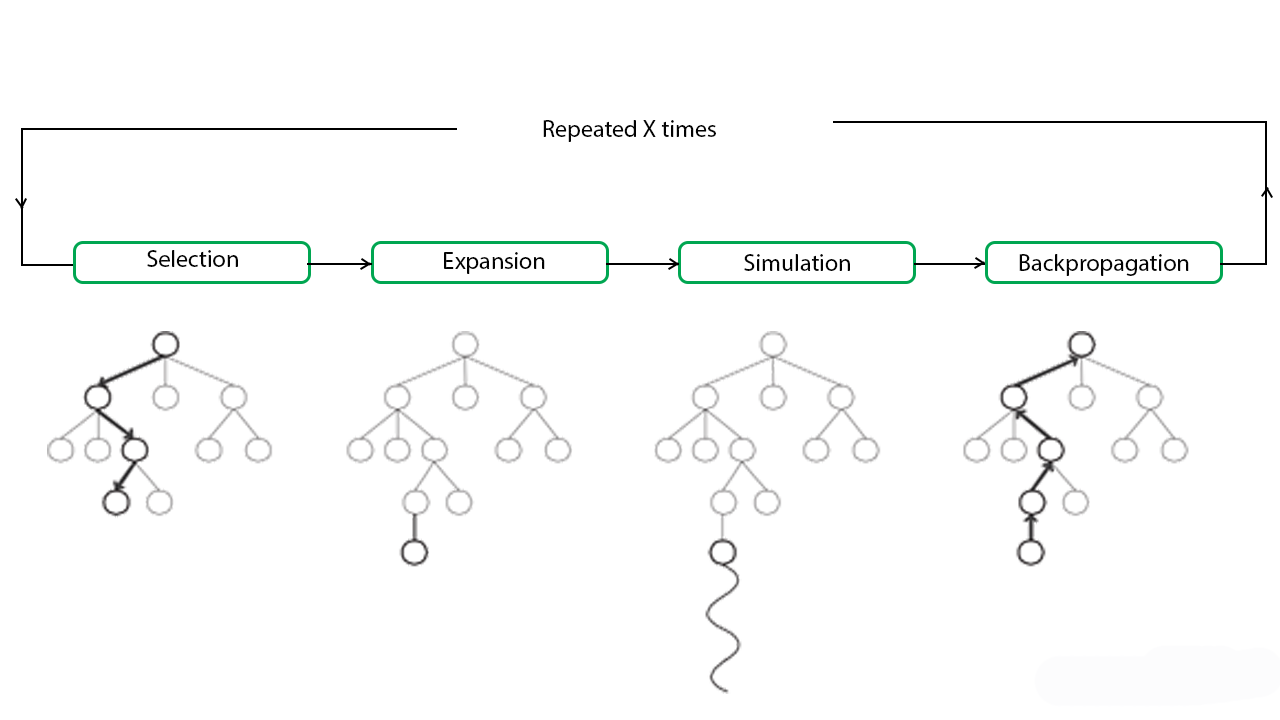
\includegraphics[width=0.9\textwidth]{obrazky-figures/mcts}
	\caption{Diagram jednotlivých fází MCTS.\@
  Zdroj:~\cite{mcts_geeksforgeeks}}\label{fig:mcts}
\end{figure}
\pagebreak
\begin{myitemize}
  \item \textbf{\emph{Selekce}}

  Na základě aktuálního stavu se vybere další stav k~prozkoumání.
  Pro tento výběr se využívají dvě strategie:
  
  \textbf{\emph{Strom s~horní mezí spolehlivosti}} (Upper confidence bounds applied to trees, UCT) kombinuje průměrnou hodnotu uzlu a~odměnu za exploraci.

  \label{epsilon_greedy}
  textbf{\emph{Chamtivá strategie $\epsilon$ }} ($\epsilon$-greedy strategy) vybírá s~pravděpodobností $\epsilon$ náhodný uzel, jinak volí uzel s~nejvyšší hodnotou.
  Tato strategie se používá méně často než UCT\@.

  Obě tyto strategie se snaží o~rovnováhu mezi explorací a~exploatací.
  \item \textbf{\emph{Expanze}}

  V~tomto kroku se vyhledávací strom rozšíří o~nový uzel, který je výstupem z~předchozího kroku.

  \item \textbf{\emph{Simulace}}

  Po této fázi je provedena náhodná simulace od nového uzlu až do konečného stavu.

  \item \textbf{\emph{Aktualizace}}
  
  Díky nově nabytým informacím ze simulace se zpětnou propagací aktualizují hodnoty uzlů ve stromě.
\end{myitemize}


Tento algoritmus se skvěle hodí na hry s~nedokonalou či neúplnou informací, jelikož se spoléhá na vzorkování pomocí simulací.

\section{Q-learning}\label{subsec:q-learning}

Q-learning je jedním z~nejznámějších algoritmů posilovaného učení.
Učení tohoto algoritmu probíhá bez modelu (model-free) a~mimo strategii (off-policy), což znamená, že se učí přímo z~interakce s~prostředím a~nezávisle na strategii, kterou agent používá k~volbě akcí.

Jak už název vypovídá, Q-learning se zaměřuje na určení hodnoty hodnotové funkce akce $Q(s, a)$, viz \ref{subsubsec:q_function}.
Tyto hodnoty se uchovávají v~Q--tabulce, která na každou kombinaci stavu a~akce uchovává hodnotu $Q(s, a)$.
Hodnoty v~Q--tabulce se iterativně aktualizují na základě získaných odměn.
Pokud agent obdrží kladnou odměnu po vykonání akce $a$ ve stavu $s$, zvýší se hodnota $Q(s, a)$.
Naopak dostane-li po vykonání této akce zápornou odměnu, hodnota $Q(s, a)$ se sníží.

Řádky Q-tabulky tedy reprezentují stavy a~sloupce akce.
Po vytvoření jsou všechny $Q$ hodnoty v~tabulce inicializovány na nulu.
Následně jsou tyto hodnoty iterativně aktualizovány dle zpětné vazby udělené od prostředí ve formě odměny.

Jako u~většiny algoritmů je zde potřeba dohlédnout na rovnováhu mezi explorací a~exploatací.
K~tomu se využívá $\epsilon$--greedy strategie viz \ref{epsilon_greedy}.

\begin{algorithm}[H]
  \caption{Učení Q-learning s~využitím $\epsilon$-greedy strategie}
  \begin{algorithmic}[1]
  \State V~Q tabulce inicializuj všechny hodnoty na 0
  \State Inicializace $\epsilon$ na 1
  \For{každou epizodu}
    \While{není dosaženo konečného stavu}
          \State S~pravděpodobností $\epsilon$ vyber náhodnou akci, jinak vyber akci s~nejvyšší hodnotou $Q(s, a)$
          \State Proveď akci $a$, pozoruj odměnu $r$ a~další stav $s'$
          \State Aktualizuj hodnotu $Q(s, a)$:\par
          $Q(s, a) = Q(s, a) + \alpha \left( r + \gamma \max_{a'} Q(s', a') - Q(s, a) \right)$
    \EndWhile
  \EndFor
  \end{algorithmic}
\end{algorithm}

\begin{myitemize}
  \item $\alpha$ -- rychlost učení
  \item $\gamma$ -- diskontní faktor
  \item $Q(s, a)$ -- hodnota akce $a$ ve stavu $s$
  \item $r$ -- odměna
  \item $s$ -- stav
  \item $a$ -- akce
  \item max$_{a'}Q(s', a')$ -- maximální hodnota budoucí odměny, pokud se agent nachází ve stavu $s'$ a~zvolí nejlepší dostupnou akci $a'$ (hodnota nejlepší akce v~následujícím stavu)
\end{myitemize}

Hlavní nevýhodou tohoto algoritmu je právě jeho závislost na Q--tabulce.
Tabulka mapuje hodnoty pro každou kombinaci stavu a~akce.
Je-li však stavový či akční prostor příliš velký, nebo dokonce nekonečný, je tento algoritmus nevhodný, téměř až nepoužitelný.
Výsledná Q tabulka by byla neefektivní kvůli své velikosti.
Mohlo by se stát, že s~nekonečným množstvím kombinací by velikost tabulky rostla do \uv{nekonečna}.
Jako řešení byl navržen algoritmus Deep Q-learning.

\section{Deep Q-learning (DQN)}\label{subsec:deep-q-learning}

Tato metoda je rozšířením algoritmu Q-learning, který nahrazuje $Q$--tabulku neuronovou sítí určenou k~aproximaci hodnotové funkce akce $Q(s, a)$.
Díky této aproximaci je možné použít tento algoritmus na problémy s~velkým či nekonečným množstvím kombinací akcí a~stavů.
Při vytvoření neuronové sítě jsou váhy inicializovány náhodně.

Avšak tímto vzniká nový problém, \emph{nestabilita učení}.
Ten je řešen dvěma mechanismy:

\begin{myitemize}
  \item \textbf{Přehrání zkušenosti (experience replay)}
  
  Během trénování se ukládají všechny zkušenosti (přechody) do paměti.
  Zkušenost zahrnuje stav, akci, odměnu a~následující stav.
  Při aktualizaci vah při trénování se náhodně vybírají skupiny zkušeností z~této paměti a~aktualizují se podle nich váhy sítě.
  Tímto se snižuje rozdíl mezi jednotlivými aktualizacemi a~tím pádem se zvyšuje stabilita učení.

  \item \textbf{Periodická aktualizace}

  Používají se dvě neurnové sítě, jedna hlavní a~jedna cílová.
  Hlavní síť se aktualizuje při každém kroku.
  Cílová síť se používá k~výpočtu hodnoty $Q(s, a)$ a~aktualizuje se méně často než hlavní síť.
  Aktualizace cílové sítě se provádí periodicky a~kopírováním hlavní sítě.
  Tímto se změny v~chování hlavní sítě nepřenášejí okamžitě do cílové sítě a~tím se zvyšuje stabilita učení.

\end{myitemize}

\begin{algorithm}[H]
  \caption{Učení Deep Q-learning s~využitím $\epsilon$-greedy strategie, pamětí zkušeností a~periodickou aktualizací cílové sítě}
  \begin{algorithmic}[1]
    \State Hlavní neuronové síti $Q$ inicializuj váhy ($\theta$) náhodně
    \State Cílovou neuronovou síť $Q^{-}$ inicializuj váhy jako kopii hlavní sítě: $\theta^{-} = \theta$
    \State Inicializace $\epsilon$ na 1
    \For{každou epizodu}
      \For{každý krok epizody}
            \State S~pravděpodobností $\epsilon$ vyber náhodnou akci, jinak vyber akci s~nejvyšší hodnotou $Q(s, a; \theta)$
            \State Proveď akci $a$, pozoruj odměnu $r$ a~další stav $s'$
            \State Ulož přechod $(s, a, r, s')$ do paměti $D$
            \If{paměť zkušeností $D$ obsahuje dostatek vzorků}
              \State Vzorkuj náhodnou skupinu přechodů $(s_j, a_j, r_j, s_j')$ z~$D$
              \For{každý vzorkovaný přechod $(s_j, a_j, r_j, s_j')$}
                  \State \textbf{Cílová hodnota $y_j$:}
                  \[
                  y_j = 
                  \begin{cases} 
                  r_j & \text{pokud je } s_j' \text{ konečný stav} \\
                  r_j + \gamma \max_{a'} Q^{-}(s_j', a'; \theta^{-}) & \text{jinak}
                  \end{cases}
                  \]
                  \State Vypočítej ztrátu a~pomocí gradientního vzestupu (gradient ascend) aktualizuj váhy hlavní sítě~$\theta$:
                   \[
                  L(\theta) = \left(y_j - Q(s_j, a_j; \theta)\right)^2
                  \]
              \EndFor
            \EndIf
            \State Každých $N$ kroků aktualizuj cílovou síť $\theta^{-}$ kopírováním hlavní sítě~$\theta$
      \EndFor
    \EndFor
  \end{algorithmic}
\end{algorithm}
\begin{myitemize}
  \item \(\theta\) --- váhy hlavní neuronové sítě \(Q\)
  \item \(\theta^{-}\) --- váhy cílové neuronové sítě \(Q^{-}\)
  \item $D$ --- paměť zkušeností
  \item $N$ --- perioda aktualizace cílové sítě
  \item $\gamma$ --- diskontní faktor
  \item $\gamma \max_{a'} Q^{-}(s_j', a'; \theta^{-})$ --- hodnota $Q$ funkce pro nejlepší akci $a'$ v~následujícím stavu $s_j'$, vypočítaná pomocí cílové sítě $Q^{-}$
  \item $Q(s_j, a_j; \theta)$ --- hodnota $Q$ funkce pro akci $a_j$ ve stavu $s_j$, vypočítaná hlavní neuronovou sítí $Q$
  \item $L(\theta) = \left(y_j - Q(s_j, a_j; \theta)\right)^2$ --- rozdíl mezi cílovou hodnotou $y_j$ a~hodnotou, kterou vypočítala neuronová síť $Q(s_j, a_j; \theta)$
  \item Hodnoty vah neuronové sítě se upraví tak, aby se minimalizovala ztráta $L(\theta)$
\end{myitemize}
\section{Metody gradientu politiky}\label{subsec:gradientni_metody}
Předchozí metody se snažily naučit či aproximovat hodnotovou funkci akce a~vždy volily tu nejlepší, to ale vede k~deterministické strategii.
Často je ale optimální stochastická strategie.
Algoritmy z~této skupiny se snaží naučit strategii přímo, a~to tím způsobem, že upravují parametry strategie, aby maximalizovaly účelovou funkci (objective function).
Nejčastěji se využívá neuronová síť, která má na vstupu stav prostředí, na výstupu pravděpodobnostní rozdělení nad akcemi a~váhy neuronů jsou právě parametry politiky.
Výsledkem metod této skupiny je tedy pravděpodobnostní rozdělení nad akcemi v~daném stavu, což znamená, že každá akce má šanci na zvolení.

Účelová funkce je tedy očekávaná odměna při následování strategie a~hodnotí strategii.
Základní účelová funkce je definována takto:
\begin{equation}
    \label{eq:ucelova_funkce_spojita}
  \mathcal{J}(\theta) = \sum_{s \in \mathcal{S}} d_{\pi_\theta}(s) V_{\pi_\theta}(s)
  \end{equation}

\begin{myitemize}
  \item $\mathcal{J}(\theta)$ -- Účelová funkce.
  \item $d_{\pi_\theta}(s)$ -- distribuční rozdělení stavů. Značí pravděpodobnost, že se agent nachází ve stavu $s$, při následování strategie $\pi_\theta$.
  \item $V_{\pi_\theta}(s)$ -- hodnota stavu $s$ při následování strategie $\pi_\theta$.\par
  \item Účelová funkce je tedy součtem hodnot stavů násobených jejich pravděpodobností výskytu.
\end{myitemize}

Hodnotu stavu $V_{\pi_\theta}(s)$ lze dále rozepsat, vznikne tedy výsledná rovnice účelové funkce:
\begin{equation}
  \mathcal{J}(\theta) = \sum_{s \in \mathcal{S}} \Big( d_{\pi_\theta}(s) \sum_{a \in \mathcal{A}} \pi(a \vert s, \theta) Q_\pi(s, a) \Big)
\end{equation}

\begin{myitemize}
  \item $\pi(a \vert s, \theta)$ --- pravděpodobnost volby akce $a$ ve stavu $s$ podle strategie $\pi_\theta$.
  \item $Q_\pi(s, a)$ --- očekávaná odměna, pokud se ve stavu $s$ zvolí akce $a$.
\end{myitemize}

\pagebreak

\subsection{Věta o~gradientu strategie a~aktualizace parametrů}
Aby bylo možné zjistit, jakým způsobem upravit parametry strategie k~maximalizaci účelové funkce, je potřeba vypočítat \emph{\textbf{gradient}\footnote[2]{Gradient značí směr funkce, značí se symbolem $\nabla_{\phi}$. Počítá se parciální derivací účelové funkce podle $\phi$.}} -- $\nabla \mathcal{J}(\theta)$.

Základní výpočet tohoto gradientu je závislý jak na pravděpodobnosti výběru akce (která je přímo určena strategií), tak na distribučním rozdělení stavů (která je nepřímo určena politikou).

Efekt změn parametrů strategie na zvolené akce lze jednoduše spočítat, ale odhadnout jejich vliv na distribuční rozdělení stavů je složité.\\
\emph{Věta o~gradientu strategie}~\cite{NIPS1999_464d828b} výrazně zjednodušuje výpočet gradientu tím, že odstraňuje derivace distribučního rozdělení stavů v~závislosti na změněných parametrech strategie:

\begin{equation}
    \label{eq:veta_o_gradientu_strategie}
    \begin{split}
        \nabla_\theta J(\theta) 
        &= \nabla_\theta \sum_{s \in \mathcal{S}} d^\pi(s) \sum_{a \in \mathcal{A}} Q^\pi(s, a) \pi_\theta(a \vert s) \\
        &= \sum_{s \in \mathcal{S}} d^\pi(s) \sum_{a \in \mathcal{A}} Q^\pi(s, a) \nabla_\theta \pi_\theta(a \vert s) 
    \end{split}
\end{equation}

\begin{myitemize}
  \item $\nabla_\theta \pi_\theta(a \vert s)$ -- gradient pravděpodobnosti volby akce $a$ ve stavu $s$ podle strategie $\pi_\theta$.
  Lze rozepsat jako: $\frac{\partial \pi_\theta(a \vert s)}{\partial \theta}$.
\end{myitemize}

Tento teorém je základem pro všechny metody gradientu politiky.
Parametry strategie se mohou upravovat například pomocí metody \textbf{gradientního  vzestupu} (gradient ascend):
\begin{equation}
  \theta_{k+1} = \theta_k + \alpha \nabla_\theta J(\theta)
\end{equation}

\begin{myitemize}
  \item $\theta_{k+1}$ -- nové parametry strategie.
  \item $\theta_k$ -- aktuální parametry strategie.
  \item $\alpha$ -- rychlost učení, standardně se volí malá hodnota okolo $0.01$.
  \item $\nabla_\theta J(\theta)$ -- gradient účelové funkce, popsaný výše.
\end{myitemize}

Nejzákladnější metodou gradientu politiky je \textbf{REINFORCE}.
Metoda je velmi podobná algoritmu Monte Carlo, ale využívá gradientu strategie k~naivní aktualizaci parametrů.
Vypočtený gradient se využije k~aktualizaci parametrů strategie, ale změna není nijak omezována.
Změny tak mohou být velmi velké, učení tak může být nestabilní, to řeší následující algoritmy.

\pagebreak

\subsection{Trust Region Policy Optimization (TRPO)}\label{sec:trust-region-policy-optimization}
Trénování strategií pomocí výpočtu gradientu je velmi náchylné na změny, kde velká a~náhlá změna v~jednom kroku může způsobit zásadní změny v~chování agenta a~omezit další učení optimálnější strategie.
Během učení totiž chceme, aby probíhalo plynule, ne skokově.
Pokud se strategie změní příliš rychle, protože následovala nejstrmější směr růstu (gradient), může se stát, že mine cestu vedoucí k~optimální strategii a~uvízne v~lokálním optimu.

TRPO je optimalizační algoritmus, který se snaží tento problém řešit tím, že definuje omezení rozdílu mezi novou aktualizovanou strategií \textbf{$\pi$} a~starou strategií kroku \textbf{$\pi_{\text{old}}$}.
Tento rozdíl mezi dvěma pravděpodobnostními rozděleními je definován jako Kullback-Leiblerova divergence (K-L divergence)\cite{KL_divergence}.

Vzniká tak region důvěry (trust region), ve kterém musí nová strategie setrvat.
Strategie se tedy nemůže skokově změnit na lokální maximum, ale pouze následuje směr gradientu.

Účelová funkce je definována jako:
\begin{equation}
  J^{TRPO}(\theta) = \sum_{s \in \mathcal{S}} d_{\pi_{\theta_{\text{old}}}}(s) \sum_{a \in \mathcal{A}} \pi_{\theta}(a \vert s) \hat{A}_{\theta_{\text{old}}}(s, a)
\end{equation}

\begin{myitemize}
  \item $\hat{A}_{\theta_{\text{old}}}(s, a)$ -- odhad výhody akce $a$ ve stavu $s$. Měří, jak je daná akce lepší než průměrná akce ve stavu $s$. Lze dále rozepsat jako: $Q_{\pi_{\theta_{\text{old}}}}(s, a) - V_{\pi_{\theta_{\text{old}}}}(s)$,
\end{myitemize}
kde rozdíl mezi novou a~starou politikou je omezen K-L divergencí:
\begin{equation}
  \label{eq:kl_divergence}
    D_{KL}(\pi_{\theta_{\text{old}}} \Vert \pi_{\theta}) \le \delta
\end{equation}

K~výpočtu nových parametrů se již nepoužívá gradientní vzestup, ale používají se Hessovy matice.
Hessova matice je vždy čtvercového tvaru.
Její hodnoty obsahují druhé parciální derivace funkce a~popisují tím její lokální zakřivení.
Tím, že se hledá lokální maximum pouze v~oblasti důvěry, problém se stabilitou je značně redukován.

Díky tomuto řešení se učení stává robustním a~stabilním.
Avšak výměnou za to je náročnost výpočtu pomocí Hessových matic a~s~tím související náročnost na implementaci.

\subsection{Optimalizace proximální strategie (PPO)}
\label{sec:proximalni-optimalizace-strategie}

Metoda optimalizace proximální strategie (Proximal policy optimization --- PPO) byla představena roku 2017~\cite{PPO_paper}.
Tato metoda je vylepšeným následníkem algoritmu TRPO, popsaným v~předchozí sekci~\ref{sec:trust-region-policy-optimization}.

Co výrazně odlišuje tuto metodu od předchůdců, je její jednoduchost a~efektivita.
Dosahuje lepších výsledků než metoda TRPO a~srovnatelných výsledků s~metodou ACER\@.
Je však mnohem jednodušší na implementaci, má nižší nároky na výkon a~je mnohem lepš, co se týče efektivity dat pro trénování~\cite{PPO_paper}.
K~dosažení těchto výsledků využívá PPO techniku ořezávání náhradních cílů vloženou do algoritmu TRPO\@.
Vynucuje, aby K-L divergence staré a~nové strategie byla v~rozmezí $[1-\epsilon, 1+\epsilon]$ kde $\epsilon$ je modifikovatelný parametr.

\pagebreak

Nechť $r(\theta)$ je pravděpodobnostní poměr mezi novou a~starou strategií.
\begin{equation}
  r(\theta) = \frac{\pi_\theta(a_t \vert s_t)}{\pi_{\theta_{\text{old}}}(a_t \vert s_t)}
\end{equation}

Pokud tento vzorec dosadíme do rovnice pro výpočet účelové funkce v~algoritmu TRPO, vznikne následovná rovnice:

\begin{equation}
    J^{CPI}(\theta) = \sum_{s \in \mathcal{S}} d_{\pi_{\theta_{\text{old}}}}(s) \sum_{a \in \mathcal{A}} \pi_{\theta}(a \vert s) r(\theta) \hat{A}_{\theta_{\text{old}}}(s, a)
\end{equation}

Nyní ale čelíme stejnému problému jako na začátku, kde při gradientním vzestupu může být změna příliš velká.
Proto tuto účelovou funkci upravíme a~zavedeme ořezávání (clipping).

\begin{equation}
  J^{\text{CLIP}}(\theta) = \sum_{s \in \mathcal{S}} d_{\pi_{\theta_{\text{old}}}}(s) \sum_{a \in \mathcal{A}} \pi_{\theta_{\text{old}}}(a|s) \min \left( r(\theta) \hat{A}_{\theta_{\text{old}}}(s, a), \, \text{clip} \left( r(\theta), 1 - \epsilon, 1 + \epsilon \right) \hat{A}_{\theta_{\text{old}}}(s, a) \right)
\end{equation}

Jelikož je toto nejdůležitější rovnice z~celé prace, znovu zadefinujeme i~známé proměnné.
\begin{myitemize}
  \item $\sum_{s \in \mathcal{S}}$ -- suma přes všechny stavy
  \item $d_{\pi_{\theta_{\text{old}}}}(s)$ -- distribuční rozdělení stavů. Značí pravděpodobnost, že se agent nachází ve stavu $s$, při následování strategie $\pi_{\theta_{\text{old}}}$.
  \item $\sum_{a \in \mathcal{A}}$ -- suma přes všechny akce
  \item $\pi_{\theta_{\text{old}}}(a|s)$ -- pravděpodobnost volby akce $a$ ve stavu $s$ podle staré strategie $\pi_{\theta_{\text{old}}}$
  \item $r(\theta)$ -- pravděpodobnostní poměr mezi novou a~starou strategií
  \item $\hat{A}_{\theta_{\text{old}}}(s, a)$ -- odhad výhody akce $a$ ve stavu $s$,\\vypočtený vzorcem: $Q_{\pi_{\theta_{\text{old}}}}(s, a) - V_{\pi_{\theta_{\text{old}}}}(s)$
  \item $\epsilon$ -- hyperparametr ořezávání
  \item clip -- funkce, která ořízne hodnotu $r(\theta)$ v~intervalu $(1 \minus \epsilon, 1+\epsilon)$
  \item min -- funkce, která vybere menší z~dvou hodnot
\end{myitemize}
V~rovnici se objevuje minimum, to bere menší z~ořezané a~neořezané hodnoty.
Volí minimum, protože jedná pesimisticky (pessimistic bound), a~tím volí nejbezpečnější možnost pro aktualizaci parametrů.

\begin{figure}[H]
	\centering
	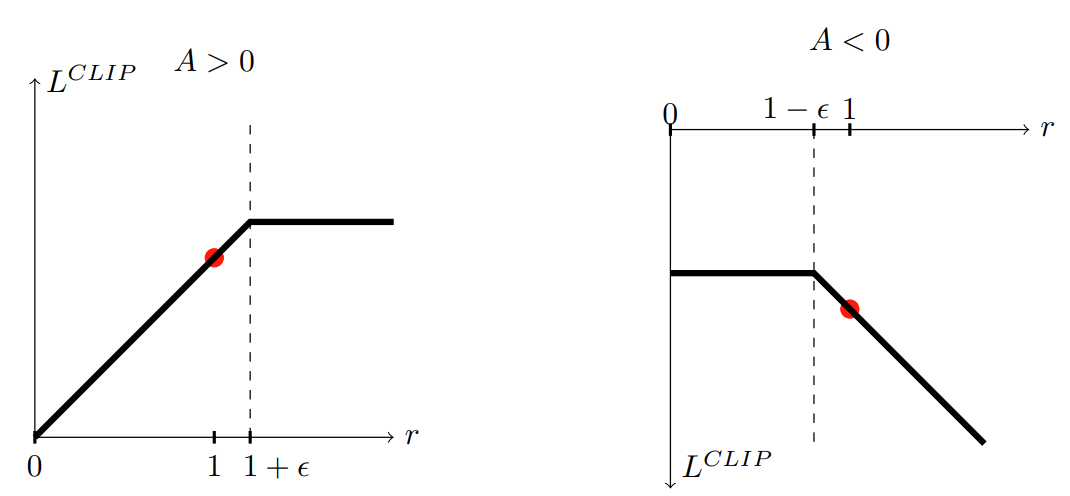
\includegraphics[width=0.6\textwidth]{obrazky-figures/clip}
	\caption{Grafy zobrazují, jak se chová funkce \emph{clip}.
  Červeným bodem je označen počáteční stav.
  Levý graf zobrazuje kladný růst gradientu, kde je tedy tento růst omezen.
  Pravý graf zobrazuje záporné klesání gradientu, kde je toto klesání omezeno.
  Zdroj:~\cite{RL_basics}}\label{fig:clip}
\end{figure}

Všechny výše uvedené vzorce byly kvůli zaměření této práce uvedeny pro diskrétní stavový i~akční prostor.
PPO však skvěle zvládá i~spojité prostory, v~případě spojitých prostorů se v~rovnicích místo sum přes všechny stavy a~akce využije \emph{očekávaná (střední) hodnota}.


Tyto změny tvoří PPO oproti TRPO kompatibilní s~metodou gradientního vzestupu, která je oproti výpočtu přes Hessovy matice velice snadná na výpočet.
Parametry se tedy aktualizují dle tohoto vzorce

\begin{equation}
  \theta_{k+1} = \theta_k + \alpha \nabla_\theta J^{\text{CLIP}}(\theta)
\end{equation}

PPO má však i~své nedostatky.
\label{PPO_weakness}
Dle studie~\cite{PPO_weakness} se ukázalo, že PPO nefunguje optimálně za 3 podmínek:
\begin{enumerate}
  \item V~prostředí se spojitým prostorem akcí je nemodifikované PPO nestabilní, pokud odměna náhle zmizí mimo ohraničenou podporu.
  \item V~diskrétním akčním prostoru s~řídkými a~vysokými odměnami PPO volí neoptimální akce.
  \item V~době těsně po inicializaci je náchylné k~předčasnému volení strategie, pokud je některá z~optimálních akcí po inicializaci blízko a~snadno dosažitelná.
\end{enumerate}

Tato studie také navrhla tato řešení a~prokázala jejich účinnost.
Bod 1 a~3 je řešen buď převedením spojitého akčního prostoru na diskrétní nebo zavedením \emph{Beta parametrizace strategie}.
\emph{KL regulováním cíle} je řešen bod 2.

Podmínka číslo 1 je v~mé implementaci prostředí hry Scotland Yard implicitně neplatná, jelikož akční prostor je diskrétní.\\
Podmínka číslo 2 je řešena přidáním menších dílčích odměn.
Agenti tak získávají odměny i~za menší kroky, nejen například za vítězství/ prohru či blízkost, viz podsekce~\nameref{subsec:odmeny}.\\

\pagebreak

\begin{algorithm}
  \caption{Proximal Policy Optimization (PPO)}
  \begin{algorithmic}[1]
  \State Počáteční parametry politiky $\theta_0$, počáteční parametry hodnotové funkce $\phi_0$
  \For{iterace $= 0, 1, 2, \dots$}
      \State Shromáždi sadu trajektorií $\mathcal{D}$ spuštěním politiky $\pi_\theta$ v~prostředí
      \State Vypočítej odměny trajektorií $\hat{R}_t$
      \State Vypočítej odhady výhod $\hat{A}_t$ pomocí aktuální hodnotové funkce $V_{\phi_k}$:
      \[
      \hat{A}_t = \sum_{t'=t}^T \gamma^{t'-t} r_{t'} - V_{\phi_k}(s_t)
      \]
      \State Aktualizuj parametry politiky $\theta$:
      \[
        \theta_{k+1} = \theta_k + \alpha \nabla_\theta J^{\text{CLIP}}(\theta)
      \]
    \EndFor
  \end{algorithmic}
  \end{algorithm}
  \begin{myitemize}
    \item $\sum_{t'=t}^T$ -- sumace přes všechny kroky trajektorií.
    \item $\gamma^{t'-t} r_{t'} - V_{\phi_k}(s_t)$ -- odhad výhody akce $a_t$ ve stavu $s_t$.
    \item $k$ -- číslo iterace
    \item $r(\theta) = \frac{\pi_\theta(a_t|s_t)}{\pi_{\theta_{\text{old}}}(a_t|s_t)}$\\ -- poměr šance zvolení akce $a_t$ ve stavu $s_t$ \\ mezi novou a~předchozí politikou
    \item $\epsilon$ -- hyperparametr klipoavací funkce.
    \item $\text{clip}(r(\theta), 1-\epsilon, 1+\epsilon) \hat{A}_t$ -- klipovaná ztráta politiky
    \item $r(\theta) \hat{A}_t$ -- ztráta politiky
    \item min --  vybere nejmenší změny, aby nedošlo k~nestabilitě učení.
    \item $\hat{A}_t$ -- odhadovaná výhoda akce $a_t$ ve stavu $s_t$
    \item $\frac{1}{\left|\mathcal{D}_k\right|T}$ -- počet trajektorií v~sadě $\mathcal{D}_k$ a~počet kroků $T$ v~trajektorii
    \item $\displaystyle\sum_{\tau \in \mathcal{D}_k} \sum_{t=0}^T$ -- sumace přes všechny trajektorie v~sadě $\mathcal{D}_k$ a~všechny kroky $t$ v~trajektorii
    \item $argmax$ -- hledá takový argument, který maximalizuje funkci pomocí optimalizačních metod (Adam, nebo gradientní vzestup)
\end{myitemize}



\chapter{Implementace systému pro autonomní hraní hry Scotland Yard}
\label{ch:navrh}
V~této kapitole je popsáno navržené řešení a~výsledná implementace systému.
\section{Zkoumaná modifikovaná verze hry Scotland Yard}\label{sec:zkoumana-modifikovana-verze-hry-scotland-yard}

Tato práce využívá modifikovanou verzi hry Scotland Yard, ve které se hráči pohybují po mřížkové herní ploše ve tvaru čtverce.
Na mřížce se nachází 15$\times$15 polí.
Hráči se po těchto polích mohou pohybovat ortogonálně i~diagonálně, vždy však o~maximálně 1 pole.
Hráč se může rozhodnout nezměnit pozici a~zůstat na svém aktuálním poli.
K~pohybu nejsou potřebné žádné jízdenky.

Tato úprava vede k~tomu, že se zjednodušil stavový i~akční prostor, jelikož se hráči nemusí starat o~svoje jízdenky a~mohou se pohybovat po herní ploše libovolně.
Změny avšak nemění základní podstatu hry, zachovává neurčitost, ale značně zjednodušuje implementaci.
Díky tomuto zjednodušení klade trénování nižší nároky na výkon.

Než začne hra, náhodně se vygenerují možné pozice, na kterých mohou Pan~X a~policisté začínat.
Z~nich se následně náhodná pozice přidělí jednotlivým hráčům.
Poté začíná hra.

Hra se dělí na jednotlivá kola, ve kterých se hráči ve svých tazích střídají.
Pro hru byli zvoleni 3 policisté, protože je herní pole velké a~2 policisté by nemuseli mít možnost ho celé pokrýt.
V~kole hraje jako první Pan~X a~poté policisté již podle svého očíslování, které jim bylo náhodně přiděleno při vytvoření.
Hra končí v~okamžiku, kdy policisté chytí Pana~X, nebo když Pan~X zůstane nepolapen až do konce.

\section{Implementace uživatelského rozhraní a~herních mechanismů}\label{subsec:implementace-uzivatelskeho-rozrani-a-hernich-mechanismu}

Uživatelské rozhraní bylo vytvořeno pomocí knihovny \texttt{Pygame}.
Hra začíná v~menu, kde je momentálně možné vybrat pouze možnost sledování hry mezi dvěma agenty.
Uživatel ale může vybrat, jaký algoritmus rozhodování je použit pro jednotlivé agenty.
K~dispozici jsou algoritmy \emph{PPO}, \emph{DQN} a~náhodné chování.

\begin{figure}[H]
	\centering
	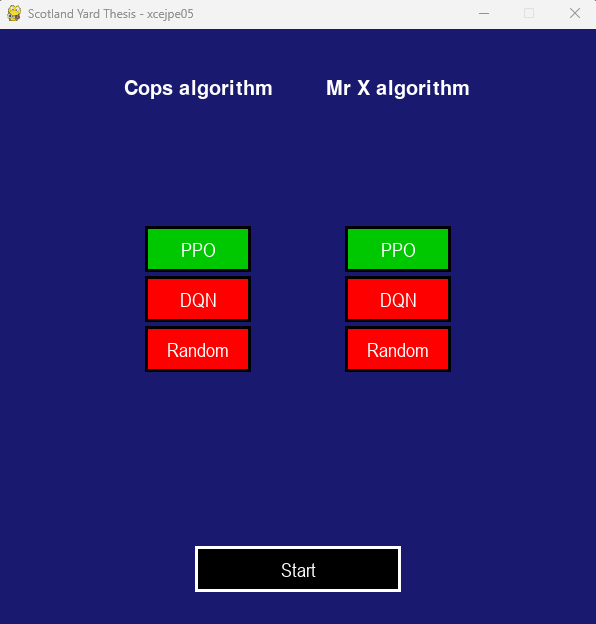
\includegraphics[width=0.7\textwidth]{obrazky-figures/game_title}
	\caption{Menu hry}\label{fig:game_title}
\end{figure}

Samotný kód hry je rozdělen na 3 části.
Jednotlivé vrstvy hry jsou tak izolovány a~mohou být snadno vyměněny za jiné verze.

\begin{myitemize}
  \item \emph{GameController}~\cite{GameSceneController}
  
  Tato třída je zodpovědná za řízení hry.
  Je zde spuštěna univerzální herní smyčka, která zpracovává uživatelské vstupy, následně provádí aktualizaci stavu aktuální scény a~její překreslení.
  \item \emph{Scény}~\cite{GameSceneController}
  
  Jednotlivé scény následně definují své chování při aktualizaci a~překreslení.
  Manipulace a~přepínání mezi nimi je zajištěno pomocí zásobníků scén.
  Do něj se ukládají nově otevřené scény a~obsluhována je vždy ta nejnovější.
  Díky tomu, když se vypne aktuální scéna, je aktivována další scéna ze zásobníku.

  \item \emph{Hra}

    Samotná hra je následovně rozdělena na 2 další části, přičemž každá zpracovává jinou část hry.
    \begin{myitemize}
      \item \emph{Herní logika} -- src/game/scotland\_yard\_game\_logic.py

      Zpracovává herní mechanismy, jako je pohyb, zpracování výherních podmínek atd.
      Zprostředkovává informace o~prostředí pro učící se agenty.
      Funkcionalita hlavní funkce \emph{step} a~jak se volí akce, je popsáno v~dalších kapitolách (\ref{subsec:neuronove_site} a~\ref{sec:system_rizeni}).

      \item \emph{Herní vizualizace} --  src/game/scotland\_yard\_game\_visual.py

      Vykreslování herních elementů (herní pole, figury atd.).
    \end{myitemize}
\end{myitemize}

\textit{Použití herní smyčky, která obsluhuje aktuální scénu, bylo inspirováno výukovým projektem z~platformy GitHub~\cite{GameSceneController}.
Kód byl ale značně upraven a~vylepšen, aby vyhovoval integrování do této práce.}

Hra se zapne v~pozastaveném stavu, aby bylo možné lépe pozorovat počáteční rozložení hráčů.
Pokud je hra pozastavena, je možné pokračovat stisknutím klávesy Space (mezerník).
Jakmile hra běží, je možné ji opětovně pozastavit stisknutím klávesy Space (mezerník).


Na herní ploše jsou zobrazeny 4 figury ve formě barevných čtverců.
Červený čtverec značí Pana~X a~zelené čtverce značí policisty.
V~levém horním rohu okna je zobrazen aktuální stav hry.
Pakliže hra stále běží, je zobrazeno číslo aktuálního kola.
Jakmile hra skončí, je zobrazeno, kdo hru vyhrál.
\begin{figure}[H]
	\centering
	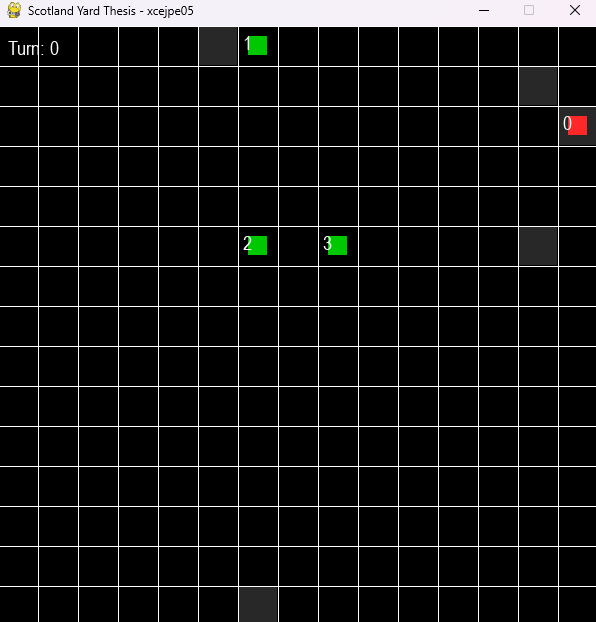
\includegraphics[width=0.8\textwidth]{obrazky-figures/game_0}
    \caption{Hra před spuštěním}
    \label{fig:game_0}
\end{figure}

V~obrázku~\ref{fig:game_0} je hra v~pozastaveném stavu a~je zobrazeno počáteční rozložení hráčů.
Na obrázku lze vidět tmavě šedé čtverce, které značí možnou pozici Pana~X\@.
Na začátku hry je těchto pozic mnoho, jelikož Pan~X doposud svoji pozici neodhalil.

\begin{figure}[H]
	\centering
	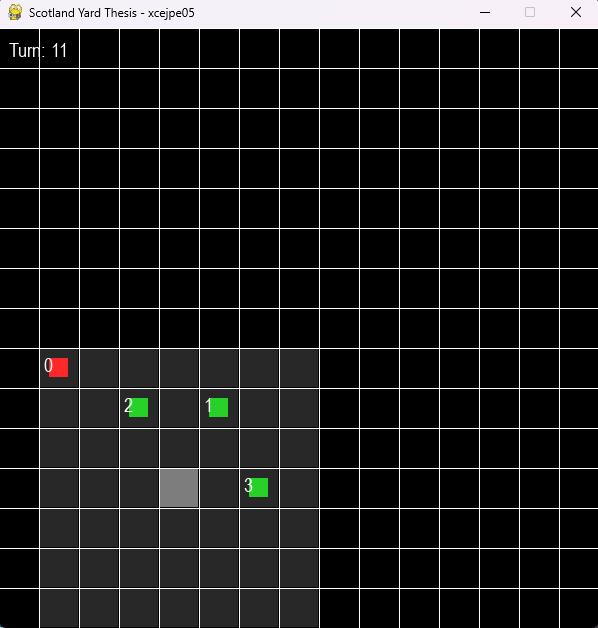
\includegraphics[width=0.8\textwidth]{obrazky-figures/game_11}
      \caption{Jedenácté kolo hry}
    \label{fig:game_11}
\end{figure}

Na obrázku~\ref{fig:game_11} je zobrazeno jedenácté kolo hry.
Světle šedý a~nejvýraznější čtverec značí poslední známou pozici Pana~X\@.
Tmavě šedé čtverce opět značí možné pozice Pana~X\@.
Na tomto obrázku lze pozorovat, že policisté jsou v~blízkosti Pana~X a~snaží se ho chytit.
Všichni policisté se z~pozic zobrazených na obrázku~\ref{fig:game_0} přesunuli na možné pozice Pana~X\@.

\section{Prostředí a~učení agentů}
\label{sec:implementace}

V~této kapitole je popsáno prostředí, ve kterém agenti vystupují, jaké informace z něj pozorují a~jaké akce mohou provádět.
Dále je popsáno, jakým způsobem byli agenti trénováni, jakou formou probíhá a~co je výsledkem tohoto trénování.


\subsection{Použitá knihova pro učení}\label{subsec:pouzite-technologie}
K~učení agentů pro hru Scotland Yard byl využit open-source framework \texttt{Ray}~\cite{Ray,liang2018rllib}.
Konkrétně byla využita knihovna \texttt{Ray.Rllib}.
Tato knihovna poskytuje nástroje pro posilované učení a~samotné implementace jednotlivých algoritmů, které byly využity v~této práci.
Rllib dokáže využívat obě populární knihovny pro strojové učení \texttt{Tensorflow} a~\texttt{Pytorch}.
Pro tuto práci byla vybrána knihovna \texttt{Pytorch}.

Knihovna \texttt{Ray} byla zvolena pro podporu učení více modelů současně, je vhodná pro velké projekty a~umožňuje možnosti konfigurace jako žádný jiný framework.
Obsahuje spoustu implementací algoritmů pro posilované učení, a~jelikož je má výsledná implementace modulární, lze jednoduše zaměnit využívaný algoritmus za jiný.

Cenou za tuto flexibilitu, modularitu a~abstrakci je ale složitost konfigurace, složitost vytvoření správného prostředí a~mnohem větší časová náročnost celého systému.
Bez výkonné grafické karty je trénování velmi pomalé.

\subsection{Pozorovací a~akční prostor agentů}
V~této práci v~prostředí vystupují dva agenti s~různými strategiemi a~různými pozorovacími prostory.
Jeden model definuje chování policistů a~druhý model ovládá chování Pana~X\@.
Akční prostor je stejný jak pro policisty, tak pro Pana~X\@.

\bigskip
\textbf{Pozorovací prostor} agentů je velmi důležitý pro úspěšné naučení dobré strategie.
Struktura jednotlivých pozorovacích prostorů je následující:

\begin{myitemize}
  \item \textbf{Shodné položky pozorování}
  \begin{myitemize}
    \item Číslo aktuálního kola;
    \item Maximální počet kol;
    \item Číslo kola, kdy dojde k~dalšímu odhalení pozice Pana~X;
    \item Počet kol, kdy agent stál na místě;
    \item Vlastní pozice agenta (x, y);
    \item Pozice (x, y) a~vzdálenost od poslední známé pozice pana~X;
    \item Pozice (x, y) zbylých policistů a~vzdálenosti od nich.
  \end{myitemize}
  \item \textbf{Pozorování, která mají policisté navíc}
    \begin{myitemize}
    \item Pozice (x, y) nejbližšího bodu oblasti zájmu;
    \item Vzdálenost od nejbližšího bodu oblasti zájmu;
    \item Pravdivostní hodnota, zda je policista v~oblasti zájmu.
  \end{myitemize}
\end{myitemize}

Agenti tedy nevidí všechna pole, ale jen ta, která jsou důležitá.
Klíčový je pozorovací prostor policistů.
Ti vidí pouze poslední známou pozici Pana~X a~\emph{oblast zájmu}, což je oblast, ve které se může Pan~X nacházet.
Tato oblast je blíže popsána v~podkapitole  \ref{subsubsec:oblast_zajmu}, kde je podrobněji vysvětlena její souvislost se systémem odměn.

Pokud informace obsažená v~těchto pozorovacích prostorech není v~daný moment definována, je nahrazena hodnotou $\minus$1.
Konkrétně se jedná pouze o~hodnoty týkající se poslední veřejně známé pozice Pana~X, jelikož v~prvních několika kolech není známa.

\begin{figure}[H]
	\centering
	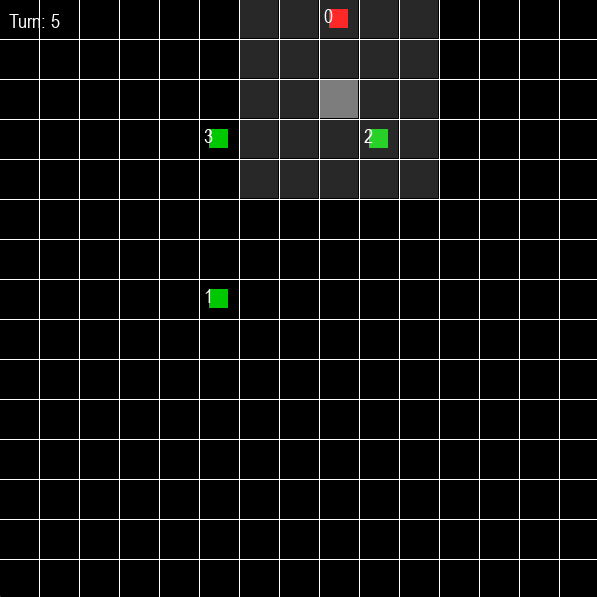
\includegraphics[width=0.8\textwidth]{obrazky-figures/game_inputs}
      \caption{Stav hry, pro ukázku vstupů do neuronové sítě}
    \label{fig:game_input}
\end{figure}
Na obrázku \ref{fig:game_input} je zobrazen stav hry.
V~tomto stavu byly jednotlivé hodnoty pozorování agentů následující:

\[
\text{mr\_x} = \begin{bmatrix}
5, & 24, & 8, & 0, & 8, & 0, & 8, & 2, & 2, & 5 \\
7, & 7.6, & 9, & 3, & 3.2, & 4, & 4, & 5.7
\end{bmatrix}
\]

\[
\text{cop\_1} = \begin{bmatrix}
5, & 24, & 8, & 0, & 5, & 7, & 8, & 2, & 5.8, & 9 \\
3, & 5.7, & 4, & 4, & 3.2, & 6, & 4, & 3.2, & 0
\end{bmatrix}
\]

\[
\text{cop\_2} = \begin{bmatrix}
5, & 24, & 8, & 0, & 9, & 3, & 8, & 2, & 1.4, & 5 \\
7, & 5.7, & 4, & 4, & 5.1, & 9, & 3, & 0, & 1
\end{bmatrix}
\]

\[
\text{cop\_3} = \begin{bmatrix}
5 & 24 & 8 & 0 & 4 & 4 & 8 & 2 & 4.5 & 5 \\
7 & 3.2 & 9 & 3 & 5.1 & 6 & 4 & 2 & 0
\end{bmatrix}
\]

\bigskip

\textbf{Akční prostor} agentů reprezentuje možné akce, které mohou agenti provést.
Tyto akce jsou stejné jak pro policisty, tak pro Pana~X\@.
Agenti se mohou hýbat ortogonálně i~diagonálně, a také můžou zůstat na místě.
Celkově tedy agent může volit z~9 akcí.

\subsection{Trénování agentů pomocí algoritmu DQN a~PPO}
Trénování je proces, při kterém agenti zlepšují své schopnosti a~strategie na základě zpětné vazby z~prostředí.
V~případě této práce agenti během učení modifikují váhy neuronů ve skrytých vrstvách neuronové sítě svého modelu, aby dosáhli požadovaného chování.

Během trénování je současně modifikován jak model pro policisty, tak model pro Pana~X\@.
Jedná se tedy o~posilované učení s~více agenty \textbf{(Marl)}.
V~tomto podoboru posilovaného učení koexistuje vícero agentů ve stejném prostředí.
Mohou mít stejné či rozdílné cíle.

V~případě této práce tedy 3 agenti reprezentují policisty se stejným cílem.
Jeden agent reprezentuje Pana~X, který má na rozdíl od zbylých agentů opačný cíl.
I~proto jsem zvolil framework Ray, který jako jeden z~mála tyto možnosti podporuje.

\subsubsection{Neuronové sítě ve výsledných modelech}
\label{subsec:neuronove_site}
V~modelech PPO i~DQN hraje hlavní roli neuronová síť.
Vstupem do těchto neuronových sítí je aktuální stav, v~případě mé práce je to viditelné pozorování agentů v~prostředí, popsané v~předchozí části.
Tyto vstupy jsou následně zpracovány skrytými vrstvami v~neuronových sítích.
Struktura vnitřních vrstev a~výstup neuronové sítě modelů jsou rozdílné pro oba algoritmy.
\bigskip

  \textbf{Neuronová síť v~modelu trénovaném algoritmem PPO}
    \begin{myitemize}
      \item Vstup
        \begin{myitemize}
          \item viditelný stav prostředí
        \end{myitemize}
      \item Struktura
        \begin{myitemize}
          \item vstupní vrstva má 17 vstupů pro Pana~X a~18 pro policisty
          \item dvě skryté vrstvy po 256 neuronech [256, 256]
          \item 9 výstupů (1 pro každou akci)
        \end{myitemize}
      \item Výstup
        \begin{myitemize}
          \item Výstupem této neuronové sítě je pravděpodobnostní rozdělení nad všemi akcemi, což znamená, že výstupem je pravděpodobnost zvolení pro každou akci, viz kapitola o~PPO \ref{sec:proximalni-optimalizace-strategie}.
          \item Jedná se tedy o~stochastickou strategii, kde každá akce má určitou šanci na zvolení, přičemž některé akce mají větší šanci a~jiné menší.
        \end{myitemize}
    \end{myitemize}

    \textbf{Neuronová síť v~modelu trénovaném algoritmem DQN}
    \begin{myitemize}
      \item Vstup
        \begin{myitemize}
          \item viditelný stav prostředí
        \end{myitemize}
      \item Struktura
        \begin{myitemize}
          \item vstupní vrstva má 17 vstupů pro Pana~X a~18 pro policisty
          \item dvě skryté vrstvy, kde první má 128 neuronů a~druhá 64 [128, 64]
          \item 9 neuronů výstupní vrstvy
        \end{myitemize}
        \pagebreak
      \item Výstup
        \begin{myitemize}
          \item Výstupem této neuronové sítě je ohodnocení všech akcí v~aktuálním stavu (hodnotová funkce Q), viz kapitola o~DQN \ref{subsec:deep-q-learning}.
          \item Používám $\epsilon$-greedy variantu, kde agent tyto hodnoty porovná a~vybere akci s~největší Q hodnotou, nebo náhodnou akci.
          Šanci na zvolení náhodné akce určuje právě $\epsilon$. Během trénování je $\epsilon$ postupně snižováno od 100\% šance na náhodnou akci k~5\% šanci na náhodnou akci.
          Vysoké epsilon vede k~exploraci a~nízké k~exploataci. Ve hře je poté $\epsilon$ nastaveno na 0%
        \end{myitemize}
    \end{myitemize}

  \bigskip

Využívám tedy implementace algoritmu PPO i~DQN, které jsou obsaženy v~knihovně \texttt{Ray.Rlib}.
PPO využívá základní parametry trénování bez žádné modifikace parametrů, jelikož se ukázalo, že agenti se chovají optimálně a~hru pochopili i~bez zásahů do výchozích hodnot hyperparametrů.
To, že nebylo třeba modifikovat parametry, je i~díky tomu, že PPO těchto hyperparametrů ani moc nemá, jeho konfigurace je tedy velmi jednoduchá oproti jiným algoritmům.

Zato DQN agenti se chovali \emph{neoptimálně} i~přes ladění hyperparametrů.
S~konfiguračními parametry \texttt{Ray.rlib}u a~hyperparametry DQN jsem dlouho experimentoval.
Měnila se velikost vnitřních vrstev, počet neuronů, rychlost učení, velikost paměti, velikost dávky učení a~další.
Agenti se i~přesto naučili pouze stát na místě, přestože toto chování bylo velmi penalizováno.
Pro vyřešení tohoto problému je nyní agentům udělována penalizace, pokud se 5 kroků po sobě nepohnou.
Penalizace je rovna zápornému počtu kol nečinnosti.
Postupně tedy roste a~pohybem je resetována.
Tato expanze odměn vedla k~vylepšení strategie agentů DQN a~nadále nestáli pouze na jednom místě.
Bohužel však přes veškeré snahy agenti DQN stále nedosahují ani zdaleka tak dobrých výsledků jako agenti PPO\@.

Trénování modelů je obsaženo v~samostatných skriptech, spustitelných z~příkazové řádky:
\begin{myitemize}
  \item TrainerDQN.py\\
  Spuštění: \texttt{python TrainerDQN.py}
  \begin{myitemize}[${}$]
    \item -{}-backup-folder [string]: složka pro záložní kopie; default: None
    \item -{}-load-folder [string]: načte model z~dané složky; default: trained\_models\_dqn
    \item -{}-save-folder [string]: uloží model do dané složky; default: trained\_models\_dqn
    \item -{}-num-iterations [int]: počet iterací trénování; default: 50
    \item -{}-save-interval [int]: interval ukládání modelu
    \item -{}-no-verbose: zákaz výpisu průběhu trénování; default: False
  \end{myitemize}
  \item TrainerPPO.py
  \item Spuštění: \texttt{python TrainerPPO.py}
  \begin{myitemize}
  \item Argumenty jsou stejné jako u~TrainerDQN.py
  \end{myitemize}
\end{myitemize}

Tyto spustitelné skripty obsahují třídy a~konfigurace pro trénování modelů.
Při spuštění skriptu se načte aktuální model, pokud existuje, a~pokračuje v~trénování tohoto modelu.
Pokud model neexistuje, je vytvořen nový model a~začíná se s~trénováním od začátku.
Model je uložen každých 5 iterací trénování.
Při dlouhém trénování doporučuji spustit script s~parametrem \texttt{-{}-do-backup}, který zároveň periodicky tvoří záložní kopie modelů.
Během několikadenního trénování může dojít k~výpadku proudu či jiné chybě a~model může být poškozen.
Během běhu skriptu se vypisuje aktuální stav trénování (pokud je nastaveno \texttt{--verbose}):
\begin{myitemize}
  \item Číslo aktuální iterace;
  \item Celkový čas trénování;
  \item Počet epizod v~iteraci a~průměrná odměna v~aktuální iteraci;
  \item U~algoritmu DQN se vypisuje aktuální hodnota epsilon.
\end{myitemize}

\subsubsection*{Řešení zvolení nevalidních akcí}
\label{subsubsec:nevalidni_akce}

Hra Scotland Yard má omezené herní pole.
Tím pádem je jasné, že pokud se hráči vyskytují na okraji herního pole, nemohou zvolit takovou akci, která by je posunula mimo toto herní pole.
Policisté také nemohou zvolit akci, která by je posunula na stejné pole, ve kterém již stojí jiný policista.
K~vyřešení tohoto problému se nejčastěji využívá tzv.~ maska akcí (\emph{Action mask}).
Framework Ray tuto možnost v~omezené míře podporuje.
Vytvořené prostředí je ale potřeba obalit v~obalové třídě, která tuto funkcionalitu zprostředkuje.
Bohužel se mi nepodařilo tuto funkcionalitu spojit s~dalšími požadavky systému, které také vyžadují zabalení do jiné třídy.
Mezi těmito požadavky je fungování více aktérů s~různými strategiemi v~jednom prostředí a~různé pozorovací prostory agentů.

Agent tedy může při trénování zvolit nevalidní akci, ale je za jejich zvolení velmi penalizován.
Agenti ji tedy volí opravdu zřídka, a~to jen na základě velmi malé explorační šance a~pouze na počátku trénování.
Pokud se i~tak stane, je ve hře implementovaná funkcionalita, která se pokusí znovu vygenerovat další akce, dokud vygenerovaná akce není validní.
Aby se zamezilo nekonečnému cyklu čekání na validní akci, je po 100 pokusech vygenerována náhodná validní akce.
Takto uměle generovaná akce nebyla za celou dobu testování agentů PPO potřeba, avšak ze statistického hlediska může tato situace nastat.

Zavedení tohoto omezení pomocí systému odměn vedlo k~positivním výsledkům a~agenti se naučili, jaké akce jsou nevalidní, a~nepoužívají je.

\subsection{Systém odměn}
\label{subsec:odmeny}

Jednotlivým agentům jsou udělovány odměny na základě jejich chování.
Jelikož policisté a~Pan~X mají odlišné a~protichůdné strategie, i~jejich odměny jsou odlišné.
Odměny, které agenti dostávají, byly navrženy odhadem a~laděny postupným experimentováním.

\bigskip

Stejné odměny, které dostávají oba agenti:
\begin{myitemize}
  \item Odměna za přímou výhru: 50 (nepřímá výhra: 30)
  \begin{myitemize}
    \item Nepřímá výhra je pro policisty, kteří se přímo nepodíleli na chycení Pana~X\@.
  \end{myitemize}
  \item Prohra: $\minus$50
  \item Nevalidní akce: $\minus$20
  \item Neaktivita: $\minus$0.5 $\times$ počet kol nečinnosti <$\minus$2.5, $\minus$12>
  \begin{myitemize}
    \item Neaktivita začíná po 5 kolech stání na místě.
    \item Tato odměna byla přidána pro podporu učení algoritmu DQN\@.
  \end{myitemize}
\end{myitemize}

\bigskip

Odměna pro Pana X navíc obsahuje:
\begin{myitemize}
  \item Vzdálenost od nejbližšího policisty: <$\minus$20, 20>
  \begin{myitemize}
    \item Odměna v~závislosti na nejbližším policistovi se ukázala jako lepší než odměna za vzdálenost od všech policistů.
    Pan X v~opačném případě tolik neřešil, když byl blízko jednoho policisty, jelikož odměna byla zprůměrována ze vzdáleností všech policistů.
  \end{myitemize}
\end{myitemize}

Odměna pro policisty navíc obsahuje:
\begin{myitemize}
  \item Vzdálenost od oblasti zájmu: <$\minus$8, 10> (Pokud je policista v~oblasti zájmu, dostává konstantní odměnu 12).
  Oblast zájmu je blíže popsána v~následující podkapitole.
\end{myitemize}

\subsubsection{Oblast zájmu}
\label{subsubsec:oblast_zajmu}

Policisté znají s~jistotou pouze poslední odhalenou pozici Pana~X\@.
Okolo tohoto bodu je vytvořena oblast zájmů, ve které se Pan~X může nacházet.
Funguje zde analogie s~reálným světem, kde při hledání osoby známe její poslední známou pozici a~její maximální rychlost a~můžeme tak vytvořit oblast, která stojí za prohledání.
Policisté vidí bod této oblasti, který je jim nejbližší, tedy vstupní bod.
Čím blíže je policista k~tomuto bodu, tím větší odměnu získává.
Pokud je od oblasti velmi vzdálený, obdrží penalizaci.
Jakmile je policista v~oblasti zájmu, dostává konstantní odměnu za to, že se v~této oblasti pohybuje.

\begin{figure}[H]
	\centering
	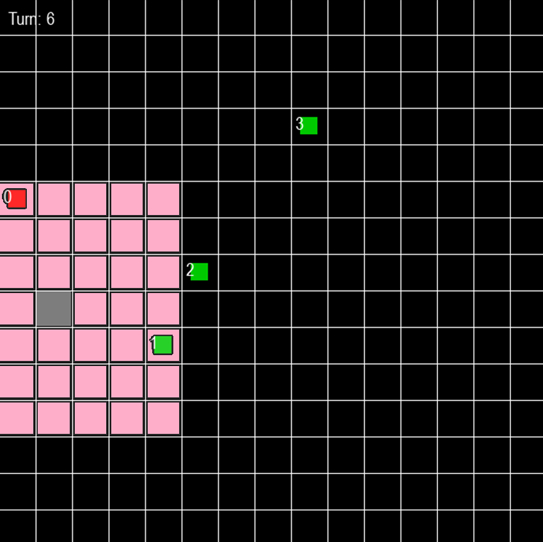
\includegraphics[width=0.6\textwidth]{obrazky-figures/interest_area}
      \caption{Zvýrazněná oblast zájmu policistů (růžově zvýrazněné pole).}
    \label{fig:game_11}
\end{figure}

PPO algoritmus může v~prostředích s~diskrétními akcemi volit velmi neoptimální akce, pokud má příliš málo podstatných odměn\cite{PPO_weakness}.
Účel této odměny je podpořit učení policistů a~zamezit tomuto problému.
Policisté tak získávají více dílčích odměn, ne pouze jednu velkou odměnu za chycení Pana~X\@.
Přidáním této dílčí odměny za interakci s~touto oblastí se výsledná strategie značně zlepšila a~agenti dosahovali lepších výsledků.

Další variantou k předání této oblasti policistům, bylo přidat do pozorování policistů pozice všech polí, kde se může Pan~X nacházet.
Toto by však bylo méně efektivní, jelikož by se pozorovací prostor výrazně zvětšil, což by zvýšilo náročnost výpočtů a~zpomalilo by se učení.
Naštěstí agenti dosahovali dobrých výsledků již se zjednodušenou variantou.

\section{Systém řízení pro hru Scotland Yard}
\label{sec:system_rizeni}
Systém řízení je zodpovědný za řízení chodu agentů a~celé hry Scotland Yard stejně jako za trénování agentů.
Systém řízení tedy můžeme rozdělit na dvě různé části podle toho, zda kontroluje trénování, nebo o~hraní hry.
V~obou variantách je hlavní smyčka, která volá hlavní metodu \textbf{step}.
Tato metoda následně volá i~metodu \textbf{play\_turn}, která řídí chod hry.

\subsection{Systém řízení během trénování}

\begin{algorithm}[H]
  \caption{\emph{step()} metoda prostředí, která se využívá při trénování}
  \label{alg:step}
  \begin{algorithmic}
    \State \textbf{vstup:} hrající agent, akce pro agenta
    \State \textbf{výstup:} pozorování pro dalšího agenta, odměna
    \State
    \If{akce je nevalidní}
    \State další agent = agent
    \State odměna = $\minus$20
    \State \textbf{return} stejný stav, odměna
    \EndIf
    \State game.play\_turn(akce)
    \State nový stav = environment.get\_state()
    \State odměna = environment.get\_reward()
    \State další agent = environment.get\_next\_player()
    \State \textbf{return} nový stav, odměna
  \end{algorithmic}
\end{algorithm}

\begin{algorithm}[H]
  \caption{Průběh trénování ve frameworku Ray}
  \label{alg:training}
  \begin{algorithmic}
    \State \textbf{vstup:} počet iterací, velikost dávky, prostředí, model
    \State \textbf{výstup:} model
    \State
    \State dávky = []
    \For{i in počet iterací}
      \For{pracovníka in pracovníci}
        \State velikost\_dávky = 0
        \State mini\_dávka = []
        \While{velikost\_dávky < max\_velikost\_dávky}
          \State stav = prostředí.získej\_stav()
          \State akce = model.získej\_akci(stav)
          \State nový stav, odměna = prostředí.step(akce)
          \State mini\_dávka.append(stav, akce, nový stav, odměna)
          \State velikost\_dávky += 1
        \EndWhile
        \State dávky.append(mini\_dávka)
      \EndFor 
      \State model.update(dávky)
    \EndFor
    \State \textbf{return} model
  \end{algorithmic}
\end{algorithm}


Za řízení trénování agentů je zodpovědný framework \texttt{Ray}.
Vícero procesů je spuštěno současně a~každý proces má svoji instanci prostředí.
Každý proces sbírá data z~hraní agentů a~následně je posílá do hlavního procesu, který je zodpovědný za zpracování těchto údajů a~trénování.
Prostředí má svoji funkci step, která je volána v~každém kroku sbírání dat.

Této metodě je předána zvolená akce dle strategie tohoto učení a~metoda zkontroluje, zda je akce validní.
Pokud je validní, prostředí ji provede.
V~opačném případě je agent penalizován za špatnou akci a~funkce step je volána znovu pro stejného agenta, dokud není zvolena validní akce.
Po provedení akce tedy metoda vypočte nový stav prostředí a~odměny za provedenou akci.
Nové pozorování z~prostředí předá dalším agentům, kteří mají hrát.
Vždy je tedy této metodě \emph{step} předána akce pro agenty, kteří obdrželi pozorování.
Tím se naznačuje, kdo hraje jako další a~kdo má čekat na svůj tah.
Tyto dávky odehraných her jsou poté předány hlavnímu procesu, který na základě použitéhu algoritmu pro učení upraví váhy své neuronové sítě, viz kapitola o~algoritmu PPO (\ref{sec:proximalni-optimalizace-strategie}) a~DQN (\ref{subsec:deep-q-learning}).

\subsection{Systém řízení během hraní hry}

\begin{algorithm}[H]
  \begin{algorithmic}
    \caption{Základní herní smyčka}
    \label{alg:GameController}
      \State scény = fronta()
      \State scény.přidej\_scénu(Úvodní\_scéna)
      \State
      \While{je fronta scén neprázdná}
        \State zpracuj\_uživatelský\_vstup()
        \If {uživatel stiskl klávesu esc}
          \State scény.odeber\_scénu()
        \EndIf
        \State scéna = scény.první\_scéna()
        \State scéna.aktualizuj\_scénu(uživatelský\_vstup)
        \State scéna.zobraz\_scénu()
      \EndWhile
  \end{algorithmic}
\end{algorithm}

Hlavní herní smyčka obsahuje frontu scén.
Scény jsou třídy, které obsahují implementace metod pro aktualizaci a~zobrazení scény.
V~této frontě jsou postupně přidávány scény, které se mají zobrazit.
Jakmile je scéna odstraněna, intuitivně se zobrazí minulá scéna.

\begin{algorithm}[H]
  \caption{Aktualizace scény hry Scotland Yard}
  \label{alg:GameScene}
  \begin{algorithmic}
    \If{hra není pozastavena}
      \State game.play\_turn()
      \If {hra skončila}
        \State Zobraz konec hry a~za 2 sekundy resetuj hru
      \EndIf
    \EndIf
  \end{algorithmic}
\end{algorithm}

\begin{algorithm}[H]
  \caption{Metoda \emph{play\_turn()}}
  \label{alg:play_turn}
  \begin{algorithmic}
    \State \textbf{vstup:} hrající agent, akce pro agenta
    \State

    \If{není akce}
      \State pocet\_pokusu = 0
      \State akce = None
      \While{je akce nevalidní}
        \If{pocet\_nevalidnich\_akci < max\_pocet\_nevalidnich\_akci}
          \State akce = model.získej\_akci(stav, agent)
          \State pocet\_nevalidnich\_akci += 1
        \Else
        \State akce = náhodná\_validní\_akce
        \EndIf
      \EndWhile
      \State \textbf{return} akce
    \EndIf
    \State agent.move(akce)
    \State agent = get\_next\_player()
  \end{algorithmic}
\end{algorithm}

Tato metoda obsluhuje jedno kolo hry.
Vstupem je agent, který má hrát, a~akce, kterou má provést.
Pokud není akce, znamená to, že neprobíhá trénování a~akci vygeneruje model.

Zde je metoda Step volána v~každém kroku  herní smyčky.
Tato metoda již nedostává akci agentů jako vstup při trénování, ale musí si ji sama vygenerovat.
Metoda step tedy volá metodu pro získání akce od hrajících agentů.

Agentům je předán aktuální stav a~ti ho pošlou na vstup neuronové sítě svého modelu a~na základě výsledků vrátí vybranou akci.
Metoda následně zkontroluje, zda je akce validní, a~pokud není, vygeneruje novou.
Samozřejmě se může teoreticky stát, že agenti budou volit nevalidní akci vždy a~program by se mohl zacyklit.
Řešení tohoto problému bylo popsáno v~kapitole \nameref{subsubsec:nevalidni_akce} (\ref{subsubsec:nevalidni_akce}).

Hlavní metoda step nyní získala akci pro agenty a~následně tuto akci provede.
Na základě jejího provedení se upraví stav prostředí a~funkce step je volána znovu, dokud nenastane konec hry.


V~průběhu realizace práce jsem experimentoval s~různými variantami průběhu kola hry:
\subsection{Prvotní verze, kde agenti hrají zároveň}
V~této verzi se hra dělila pouze na kola a~funkce step obsluhovala celé toto kolo.
Ve funkci step tedy byly volány metody pro získání akce pro všechny agenty, které se nakonec vykonaly najednou.
V~této variantě ještě nebyla přidána možnost akce stání na místě.
A~tak si Pan~X vybudoval velmi zajímavou strategii, kde místo aby se od policistů držel co nejdále, tak se k~policistům klidně přibližoval a~využíval toho, že hrají současně.
Toto zneužívání spočívalo v~tom, že vždy šel na pole, na němž již byl policista, jelikož věděl, že na daném místě již další kolo být nemůže.

Tento styl ale neodpovídal tomu jak, se skutečně hra hraje, protože všichni hráči nemohou hrát současně.
\subsection{Finální verze, kde se agenti střídají}
Zde již byla implementována možnost stání na místě a~agenti se střídají v~tahu.
Hra je tedy členěna na kola a~ta jsou dále členěna na tahy jednotlivých hráčů.
Tato verze již více odpovídá reálné hře.

\chapter{Experimenty}
\label{ch:experimenty}

Pro ověření vlastností algoritmu PPO byly provedeny dva experimenty.
Experimenty byly prováděny na systému s~následujícími parametry:

\begin{myitemize}
  \item Operační systém: Windows 10 (64-bit)
  \item Procesor: Intel Core i5--9300H
  \item Paměť: 16 GB DDR4
  \item Grafická karta: NVIDIA GeForce GTX 1660 Ti
\end{myitemize}

Agenti DQN i~PPO se učili ve stejném prostředí, za stejných počátečních podmínek, měli totožný stavový i~akční prostor a~od prostředí získávaly stejné odměny.

Pro uskutečnění těchto experimentů byly vytvořeny skripty v~jazyce Python.
Jeden pro sběr dat a~druhý pro jejich následné vyhodnocení a~zpracování do grafů a~textové podoby.

\section{Experiment 1: Pozorování vývoje chování během tréninku}
\label{sec:experiment-1}

Experiment trénování spočívá v~ukázce, jak se agenti postupem trénování zlepšují.
U~agentů DQN a~PPO je očekáván nárůst průměrné odměny a~snížení průměrné vzdálenosti policistů od Pana~X\@.
Experiment v~průběhu tréninku periodicky provádí simulace her mezi agenty a~zaznamenává jejich průběh.

\bigskip
\noindent Hlavními sledovanými parametry jsou:
\begin{myitemize}
  \item Průměrná odměna Pana~X;
  \item Průměrná odměna policistů;
  \item Průměrná vzdálenost policistů od Pana~X;
  \item Počet vyhraných her Pana~X;
  \item Počet vyhraných her policistů.
\end{myitemize}
Experiment sleduje vývoj těchto hodnot po \textbf{1000 iterací}.
To znamená, že na konci experimentu podstoupili všichni agenti přesně 1000 iterací tréninku

Simulační hry byly prováděny ve všech možných kombinacích algoritmů.
Zkoušeny tedy byly všechny algoritmy jak v~roli Pana~X, tak v~roli policistů.
Simulace byly spouštěny po různém počtu trénovacích iterací v~závislosti na aktuálním počtu již provedených iterací.\pagebreak

Počet simulací byl následovný:
\begin{myitemize}
  \item 50 simulací každých 10 iterací, do 100 trénovacích iterací;
  \item 50 simulací každých 20 iterací, od 100 do 500 trénovacích iterací;
  \item 50 simulací každých 50 iterací, od 500 do 1000 trénovacích iterací.
\end{myitemize}

Při učení je nejzajímavější sledovat vývoj chování agentů na začátku trénování.
Proto byly simulace prováděny s~větší četností právě na začátku a~postupem trénování byla četnost snižována pro snížení výpočetní a~časové zátěže simulací.
Tím bylo zajištěno, že experiment správně a~efektivně vyobrazuje, jak rychle a~jestli vůbec byli agenti schopni pochopit cíl hry.
Sběr dat pro tento experiment trval přibližně 18 hodin.
Při četnějším sběru dat by rapidně narostla časová náročnost experimentu a~dle testovacích spuštění a~výpočtů by trval i~několik dní.

\subsection{Výsledky experimentu}
\label{subsec:vysledky-experimentu-1}

Při sledování výsledků tohoto experimentu je důležité si uvědomit, že díky základní premise hry Scotland Yard je pro policisty vyhrát mnohem složitější než pro Pana~X, protože policisté dokážou vyhrát pouze tehdy, pokud chytí Pana~X, zato Pan~X může vyhrát jenom na základě uplynutí maximálního počtu kol.

Všechny následující grafy vyobrazují průměrnou odměnu Pana~X (modrá nepřerušovaná linie) a~policistů (oranžová přerušovaná linie), průměrnou vzdálenost policistů od Pana~X (zelená tečkovaná linie), a~to vše v~závislosti na počtu trénovacích iterací.

\subsubsection*{Srovnání s~náhodným agentem}
\begin{figure}[H]
  \begin{minipage}{.48\textwidth}
    \centering
    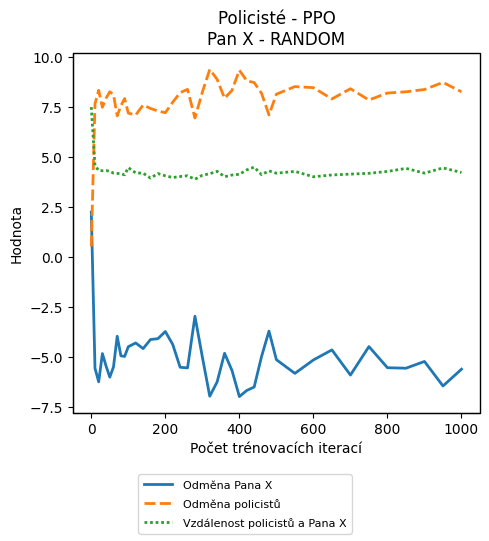
\includegraphics[width=1\textwidth]{obrazky-figures/graphs/cop_PPO_mrx_RANDOM}
    \caption{Graf simulace her mezi policisty trénovanými pomocí PPO a~Panem X volícím náhodné akce}
    \label{fig:cop_ppo_mrx_random}
  \end{minipage}\hfill
  \begin{minipage}{.48\textwidth}
    \centering
    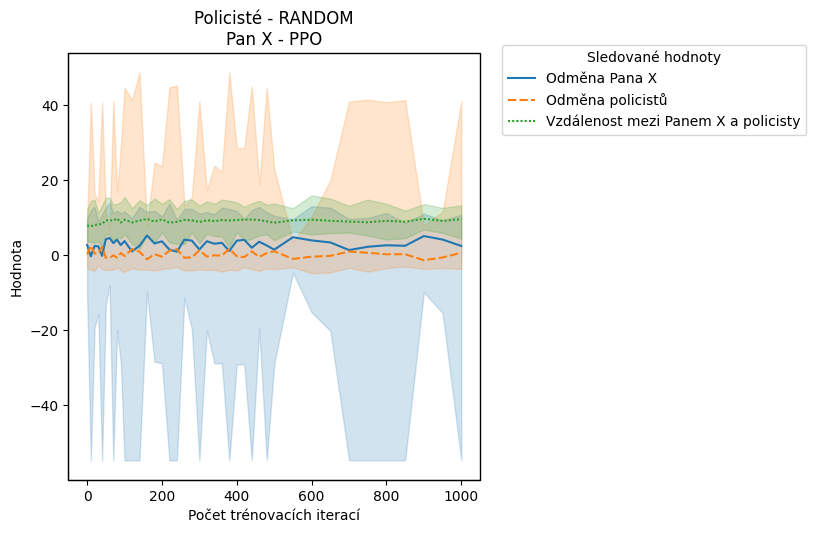
\includegraphics[width=1\textwidth]{obrazky-figures/graphs/cop_RANDOM_mrx_PPO}
      \caption{Graf simulace her mezi Panem X trénovaným pomocí PPO a~policisty volícími náhodné akce}
      \label{fig:cop_random_mrx_ppo}
  \end{minipage}
  \end{figure}

Jak lze vidět na grafu~\ref{fig:cop_ppo_mrx_random}, policisté jsou velmi úspěšní ve své strategii.
Vzdálenost mezi policisty trénovanými pomocí PPO a~Panem X, který volí náhodné akce, je po celou dobu velmi malá.
Odměna, kterou policisté získávají, je velmi vysoká.
Odměna Pana~X je naopak velmi nízká.

Na grafu lze také sledovat, že průměrná vzdálenost policistů od Pana~X na začátku trénování rapidně klesá, stejně tak klesá odměna Pana~X tím, že se zlepšuje strategie policistů.
Po tomto rapidním poklesu se vzdálenost policistů od Pana~X stabilizuje a~odměna Pana~X se drží na nízké hodnotě.

Naopak z~grafu~\ref{fig:cop_random_mrx_ppo} lze pozorovat, že je odměna Pana~X kladná a~až na odchylky vyšší než odměna policistů, kteří se chovají náhodně.
Odměna policistů se pohybuje kolem nuly a~odměna Pana~X je stále kladná.
Také vzdálenost policistů od Pana~X je skoro dvojnásobná než v~předchozím případě.

\begin{figure}[H]
  \centering
  \begin{minipage}{.48\textwidth}
    \centering
    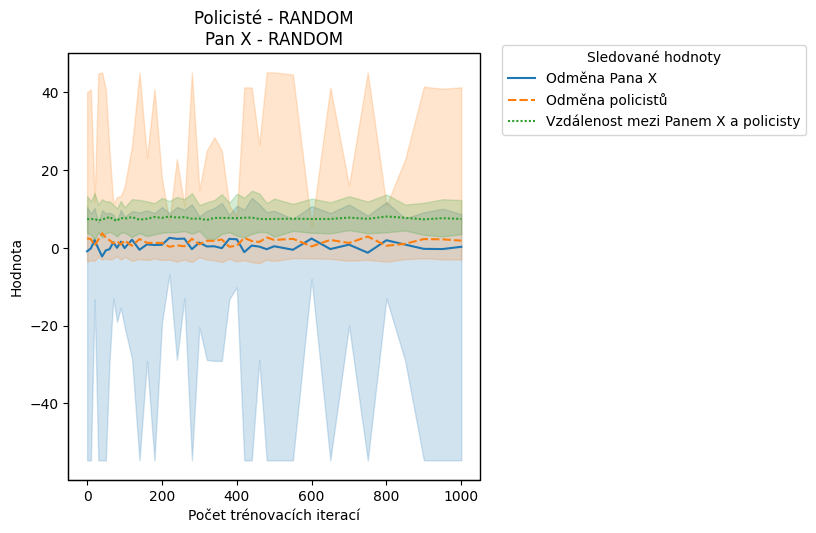
\includegraphics[width=1\textwidth]{obrazky-figures/graphs/cop_RANDOM_mrx_RANDOM}
    \caption{Graf simulace her mezi policisty a~Panem X, kde oba volí náhodné akce}
    \label{fig:cop_random_mrx_random}
  \end{minipage}\hfill
  \begin{minipage}{.48\textwidth}
    \centering
    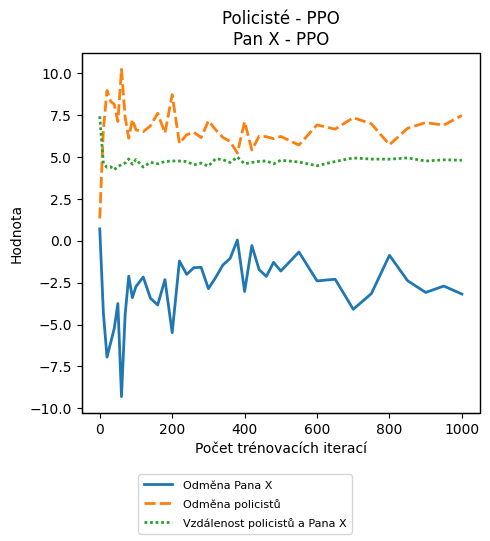
\includegraphics[width=1\textwidth]{obrazky-figures/graphs/cop_PPO_mrx_PPO}
      \caption{Graf simulace her, kde oba agenti volí akce dle modelu PPO}
      \label{fig:cop_ppo_mrx_ppo}
  \end{minipage}
  \caption{Srovnání PPO agentů s~agenty volící náhodné akce}
  \label{fig:srovnani_random_ppo}
  \end{figure}

Na srovnání~\ref{fig:srovnani_random_ppo} lze vidět, že jak PPO, tak náhodný algoritmus udržují velice stabilní vzdálenost.
U~náhodného chování je to kvůli základní pravděpodobnosti, která musí být průměrně stejná.
U~grafu agentů PPO to vypovídá o~tom, že policisté dokážou stabilně odhadovat pozici Pana~X a~přinejmenším se pohybovat v~jeho blízkém okolí.
Z~grafu \ref{fig:cop_ppo_mrx_ppo} lze pozorovat, že odměna policistů a~Pana~X kolísá.
Frekvence tohoto kolísání se postupně jemně zmenšuje.
Z~toho odvozuji, že toto kolísání vypovídá o~tom, že se agenti postupně učí strategii protivníka a~snaží se podle ní upravit svoji strategii, aby byli opět lepší.
To značí, že se obě strategie pomalu přibližují k~optimu.
Předpokládám, že dalším trénováním by se tento trend potvrdil.
Avšak k~tomu by byl zapotřebí větší výpočetní výkon a~spousta času.
Ale jak lze vidět z~výsledků experimentu, i~přes relativně malý počet trénovacích iterací se objevuje očekávané chování a~rozdíl s~náhodným chováním je markantní.

\subsubsection*{Závěr experimentu pro algoritmus PPO}

Každá možná kombinace využití algoritmů pro policisty a~Pana~X byla během experimentu testována celkově 2050$\times$.
Z~tohoto testování vzešly kromě grafů vývoje chování také údaje zaznamenávající výsledky jednotlivých her.
Tyto výsledky byly zpracovány do tabulek, které zobrazují procentuální počet výher jednotlivých stran v~závislosti na použitém algoritmu.

\begin{figure}[H]
  \centering
  \begin{minipage}{.48\textwidth}
    \begin{table}[H]
    \centering
  \begin{tabular}{@{} c|c|c|c @{}}
  \headercell{\\Policisté} & \multicolumn{3}{c@{}}{Pan~X}\\
  \cmidrule(l){2-4}
  & \multicolumn{1}{c}{PPO}&\multicolumn{1}{c}{Random}&
  \multicolumn{1}{c}{DQN} \\ 
  \hline
  PPO                                    & 38 \% & 67 \% & 65 \% \\ \hline
  Random                                    & 11 \% & 20 \% & 18 \% \\ \hline
  DQN                                    & 10 \% & 17 \% & 19 \% \\ \hline
\end{tabular}
\caption{Zobrazuje procentuální počet výher policistů proti Pánovi~X s~vybraným algoritmem během experimentu}
\label{tab:train_experiment_police_wins}    
\end{table}  
\end{minipage}\hfill
  \begin{minipage}{.48\textwidth}
    \begin{table}[H]
    \centering
    \begin{tabular}{@{} c|c|c|c @{}}
      \headercell{\\Pan~X} & \multicolumn{3}{c@{}}{Policisté}\\
      \cmidrule(l){2-4}
      & \multicolumn{1}{c}{PPO}&\multicolumn{1}{c}{Random}&
      \multicolumn{1}{c}{DQN} \\
      \hline
      PPO                                    & 62 \% & 89 \% & 90 \% \\ \hline
      Random                                    & 33 \% & 80 \% & 83 \% \\ \hline
      DQN                                    & 35 \% & 82 \% & 81 \% \\ \hline
      \end{tabular}
      \caption{Zobrazuje procentuální počet výher Pana~X proti policistům s~vybraným algoritmem během experimentu}
      \label{tab:train_experiment_mrx_wins2}
    \end{table}
  \end{minipage}
  \end{figure}

Pokud zde opět porovnáme výsledky, kdy proti sobě hráli dva náhodní agenti a~agenti trénovaní pomocí PPO, lze vidět, že agenti trénovaní pomocí PPO mají výrazně lepší výsledky.
\subsubsection{Ostatní výsledky}

\begin{figure}[H]
  \centering
  \begin{minipage}{.48\textwidth}
    \centering
    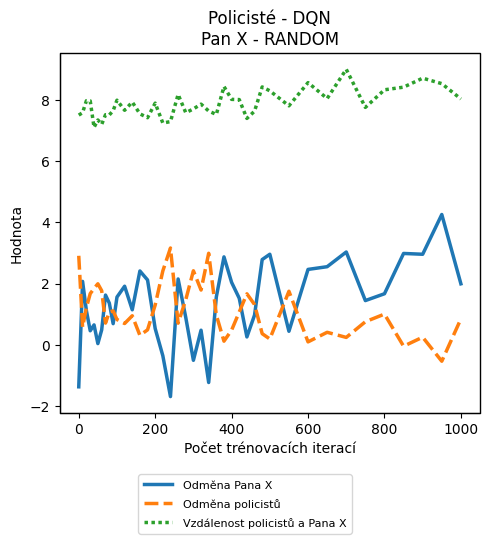
\includegraphics[width=1\textwidth]{obrazky-figures/graphs/cop_DQN_mrx_RANDOM}
    \caption{Graf simulace hry mezi policisty trénovanými pomocí DQN a~Panem X volícím náhodné akce}
    \label{fig:cop_dqn_mrx_random}
  \end{minipage}\hfill
  \begin{minipage}{.48\textwidth}
    \centering
    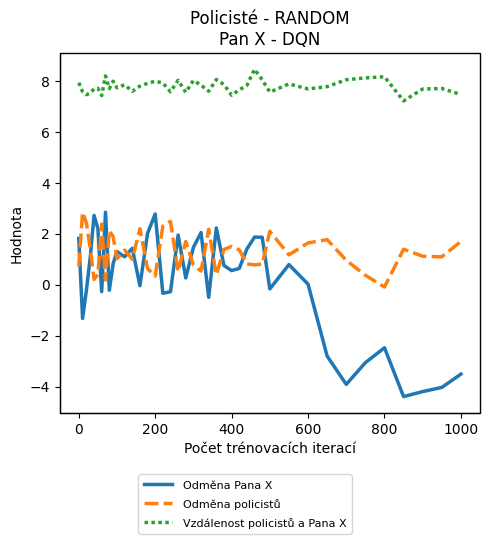
\includegraphics[width=1\textwidth]{obrazky-figures/graphs/cop_RANDOM_mrx_DQN}
      \caption{Graf simulace hry mezi Panem X trénovaným pomocí DQN a~policisty volícími náhodné akce}
      \label{fig:cop_random_mrx_dqn}
  \end{minipage}
  \label{fig:srovnani_dqn}
  \end{figure}

Jak již jsem zmiňoval, výsledky trénování agentů pomocí algoritmu DQN bohužel nemají dobré výsledky.
Výsledné chování se velmi podobá náhodnému agentovi.
Z~předchozích prací je známo, že by algoritmus DQN měl mít znatelně lepší výsledky než náhodná metoda~\cite{Hrklova2023thesis}.
Algoritmus DQN je velice citlivý na hyperparametry a~je možné, že bylo zvoleno nevhodné nastavení.
Potřebuje také mnohem více trénovacích iterací než PPO\@.
Je tedy možné, že 1000 iterací není dostatečné pro naučení dobré strategie pro algoritmus DQN\@.
Jelikož jsou ale trénovací iterace PPO časově náročnější než iterace DQN, nebylo možné sladit jejich počet.

\emph{Trénování z~tohoto experimentu poslouží jako základ pro další experiment, kde budou simulovány hry s~již natrénovanými agenty.}

\section{Experiment 2: Simulace hry s~již natrénovanými agenty}
\label{sec:experiment-2}

Tento experiment byl proveden za účelem ověření, zda jsou agenti trénovaní pomocí algoritmu PPO schopni pochopit cíl hry a~naučit se optimální strategii.
Porovnává, jestli se natrénované modely z~experimentu 1 výrazně liší od agenta, který volí pouze náhodné akce, a~tím prokázat, že se chová způsobem, který vede k~vítězství.

Pro ověření skutečného výkonu agentů byly provedeny simulace hry mezi již natrénovanými agenty.
Ačkoli již předchozí experiment dokazuje, že agenti trénovaní pomocí algoritmu PPO jsou schopni pochopit cíl hry, je důležité získat skutečná data o~výkonu jednotlivých metod bez zkreslených výsledků kvůli trénování.

Následující tabulky byly získány z 10000 simulací pro každou kombinaci již natrénovaných algoritmů.

\begin{figure}[H]
  \centering
  \begin{minipage}{.48\textwidth}
    \begin{table}[H]
    \centering
  \begin{tabular}{@{} c|c|c|c @{}}
  \headercell{\\Policisté} & \multicolumn{3}{c@{}}{Pan~X}\\
  \cmidrule(l){2-4}
  & \multicolumn{1}{c}{PPO}&\multicolumn{1}{c}{Random}&
  \multicolumn{1}{c}{DQN} \\ 
  \hline
  PPO                                    & 26 \% & 72 \% & 64 \% \\ \hline
  Random                                    & 10 \% & 19 \% & 18 \% \\ \hline
  DQN                                    & 8 \% & 17 \% & 17 \% \\ \hline
\end{tabular}
\caption{Zobrazuje procentuální počet výher policistů proti Pánovi~X s~vybraným algoritmem}
\label{tab:simulation_experiment_police_wins}    
\end{table}  
\end{minipage}\hfill
  \begin{minipage}{.48\textwidth}
    \begin{table}[H]
    \centering
    \begin{tabular}{@{} c|c|c|c @{}}
      \headercell{\\Pan~X} & \multicolumn{3}{c@{}}{Policisté}\\
      \cmidrule(l){2-4}
      & \multicolumn{1}{c}{PPO}&\multicolumn{1}{c}{Random}&
      \multicolumn{1}{c}{DQN} \\
      \hline
      PPO                                    & 74 \% & 90 \% & 92 \% \\ \hline
      Random                                    & 28 \% & 81 \% & 82 \% \\ \hline
      DQN                                    & 36 \% & 82 \% & 83 \% \\ \hline
      \end{tabular}
      \caption{Zobrazuje procentuální počet výher Pana~X proti policistům s~vybraným algoritmem}
      \label{tab:train_experiment_mrx_wins}
    \end{table}
  \end{minipage}
  \end{figure}

Z~tabulky lze vyčíst, že policisté trénovaní pomocí PPO vyhráli proti Pánovi~X s~náhodným chováním 72 \% her.
V~porovnání s~policisty volícími náhodné akce je to výrazně lepší výsledek.
Ti proti Pánovi~X s~náhodným chováním vyhráli pouze 19 \% her.

Z~her vzešly také tyto informace:
\begin{myitemize}
  \item Průměrná vzdálenost mezi Panem X a~policisty (oba PPO): 4.779692656488397;
  \item Průměrná vzdálenost mezi Panem X a~policisty (oba náhodné chování): 7.631191103120987;
  \item Průměrná vzdálenost mezi Panem X a~policisty (oba DQN): 7.869671633109524.
\end{myitemize}

Z~tohoto experimentu lze tedy vyvodit, že agenti trénovaní pomocí algoritmu PPO byli schopni se naučit optimální strategii i~ve hře s~neúplnou informací.

\chapter{Závěr}
\label{ch:zaver}

Provedené experimenty ukázaly, že algoritmus PPO je skutečně vhodný na hry s~neúplnou informací, jelikož policisté trénování pomocí PPO dokázali odhadovat přibližnou pozici Pana~X a~měli mnohem větší úspěšnost než náhodní agenti.
Agenti dokázali pochopit koncept a~cíl hry Scotland Yard.
Naučili se v~ní chovat optimálně, přestože začínali s~nulovými znalostmi o~prostředí.
Bylo příjemným překvapením, že již po pouhých 10 iteracích trénování byli agenti schopni ukazovat lepší výsledky než agent s~náhodným chováním.

\section*{Možná vylepšení}
\label{sec:mozna-vylepseni}

Bohužel se během experimentu nepovedlo separovat výslednou strategii od frameworku \texttt{Ray.Rlib} a~extrahovat ji do podoby, kde by již \texttt{Rlib} nebyl potřeba pro její využití.
Při spouštění hry se tedy načítá i~celý framework \texttt{Ray.Rlib}, toto velmi zpomaluje načítání hry, kdy prvotní načtení trvá několik sekund.
Toto a~spoustu dalších potíží jsou důvody, proč zvolení knihovny Ray.Rllib zpětně lituji.
Měl jsem spíše algoritmus PPO implementovat svépomocí s~využitím \texttt{Pytorch} či \texttt{Tensorflow}, nebo využít knihovnu \texttt{CleanRl} a~učení více strategií naráz vyřešit jiným způsobem.

\medskip
Původním plánem bylo také realizovat možnost hraní hry mezi lidmi a~agenty.
Tuto implementaci jsem ale přes problémy s~experimenty a~algoritmem DQN nestihl dokončit.
Mám za to, že by tato možnost nadále prohloubila výsledky této studie o~zajímavé experimenty, kde by bylo možné sledovat, jak si agent PPO vede proti lidskému protivníkovi.

\medskip
Agenti trénovaní pomocí algoritmu DQN měli velmi špatné výsledky.
Je vyloučeno, že by byla chyba v~prostředí, udělování odměn či v~pozorování, jelikož se agenti trénovaní pomocí PPO učili za stejných podmínek a~jejich výsledky byly dobré.
Je možné, že i~přes hledání optimálních parametrů s~pomocí \texttt{Ray.Tune} byla zvolena nevhodná konfigurace.
Byť jsem s~těmito parametry sálodlouze experimentoval, nebylo dosaženo uspokojivých výsledků.
Navrhuji změnu stavového a~akčního prostoru, aby byl kompatibilní s~verzemi studentů z~minulých let, kteří realizovali bakalářskou práci na podobné téma, a~následně využít jejich implementaci pro další experimenty~\cite{Hrklova2023thesis}.

\medskip
Dále je zde možnost rozšířit hratelnost hry o~jednotlivé druhy dopravy a~k~nim příslušící jízdenky.
Tím by výrazně vzrostla složitost hry a~stavový prostor.
Jak ale ukázala práce OpenAI~\cite{Dota2}, algoritmus PPO nemá problém s~obrovským stavovým i~akčním prostorem a~naučit se i~komplikované hry.



%===============================================================================

% Pro kompilaci po částech (viz projekt.tex) nutno odkomentovat
%\end{document}
